\section{Evaluación de propiedades de sistemas}
	Para evaluar las propiedades de los siguientes sistemas, se utilizaron las siguientes señales, de acuerdo al criterio que se buscaba evaluar:
	\begin{itemize}
		\item \textbf{Invariancia temporal:} Se utilizó un pulso cuadrado, de duración 1 \textit{s}, con amplitud 1. Luego se utiliza un pulso de las mismas características pero retrasado temporalmente en $k = 5$\textit{s}. En el caso de que ambas entradas, lleguen a la misma salida, únicamente retrasadas, el sistema es invariante en el tiempo.
		\begin{equation}
			y[n-k] = S\{ x[n-k]  \}
			\label{eq:cond_invarianza_temporal}
		\end{equation}
		
		\item \textbf{Linealidad:} Se utilizan, dos señales de ruido blanco de potencia 10 dB, las cuales se amplifican por constantes $\alpha$ y $\beta$. De esta manera, luego se aplica la definición de sistemas lineales para comprobar:
		\begin{equation}
			\alpha y_{1}[n] + \beta y_{2}[n] = S \{ \alpha x_{1}[n] + \beta x_{2}[n] \} 
			\label{eq:cond_linealidad}
		\end{equation}
		
		De esta forma, si el sistema cumple ambos lado de la igualdad, se tendrá que el sistema es lineal. Para los siguientes sistemas, se escogieron los siguientes valores para las variables:
		\begin{table}[H]
			\center
			\begin{tabular}{|c|c|}
				\hline
				\textbf{Constante} & \textbf{Valor} \\
				\hline
				$\alpha$ & 2 \\
				\hline
				$\beta$ & 3 \\
				\hline			
			\end{tabular}
			\caption{Valores para constantes para probar linealidad}
			\label{tab:lineal_const_values} 	
		\end{table}
		
		Para simplificar la notación, en los gráficos de prueba, se denomina a las entradas de ruido blanco escaladas de la siguiente forma:
		\begin{align}
			u_{1}[n] = \alpha x_{1}[n] \\
			u_{2}[n] = \beta x_{2}[n]
			\label{eq:lineality_inputs}
		\end{align}
		
		También se define las salidas esperadas, dadas la expresión en la ecuación \ref{eq:cond_linealidad}, de la siguiente manera: 
		\begin{equation*}
			\underbrace{\alpha y_{1}[n] + \beta y_{2}[n]}_{Y_{1}[n] + Y_{2}[n]} = \underbrace{S \{ \alpha x_{1}[n] + \beta x_{2}[n] \}}_{Y[n]} 
		\end{equation*}
		De esta forma, llegando a expresiones más compactas, en términos de lo que se obtuvo en matlab:
		\begin{align}
			Y[n] = S \{ u_{1}[n] + u_{2}[n] \} \\
			Y_{1}[n] = S \{ u_{1}[n] \} \\
			Y_{2}[n] = S \{ u_{2}[n] \}
			\label{eq:lineality_outputs}
		\end{align}
		
		\item \textbf{Estabilidad BIBO:} Para comprobar esta propiedad, se utiliza un delta de Kronecker, un escalón unitario  y una señal triangular de frecuencia 1 \textit{Hz}. Luego analizamos la respuesta del sistema, utilizando la siguiente definición:
		\begin{equation}
			|x[n]| \leq M_{x} < \infty \Rightarrow |y[n]| \leq M_{y} < \infty \quad \forall n
			\label{eq:cond_bibo}
		\end{equation}
		
		De esta forma, analizamos la salida del sistema frente a las entradas, y se busca comprobar que ésta sea acotada.  
	\end{itemize}

\newpage

	\subsection{Sistema \#1}
		\subsubsection{Invariancia temporal}
			Aplicando la señal de prueba en el sistema, con retardo igual a cero:
			\begin{figure}[H]
				\center
				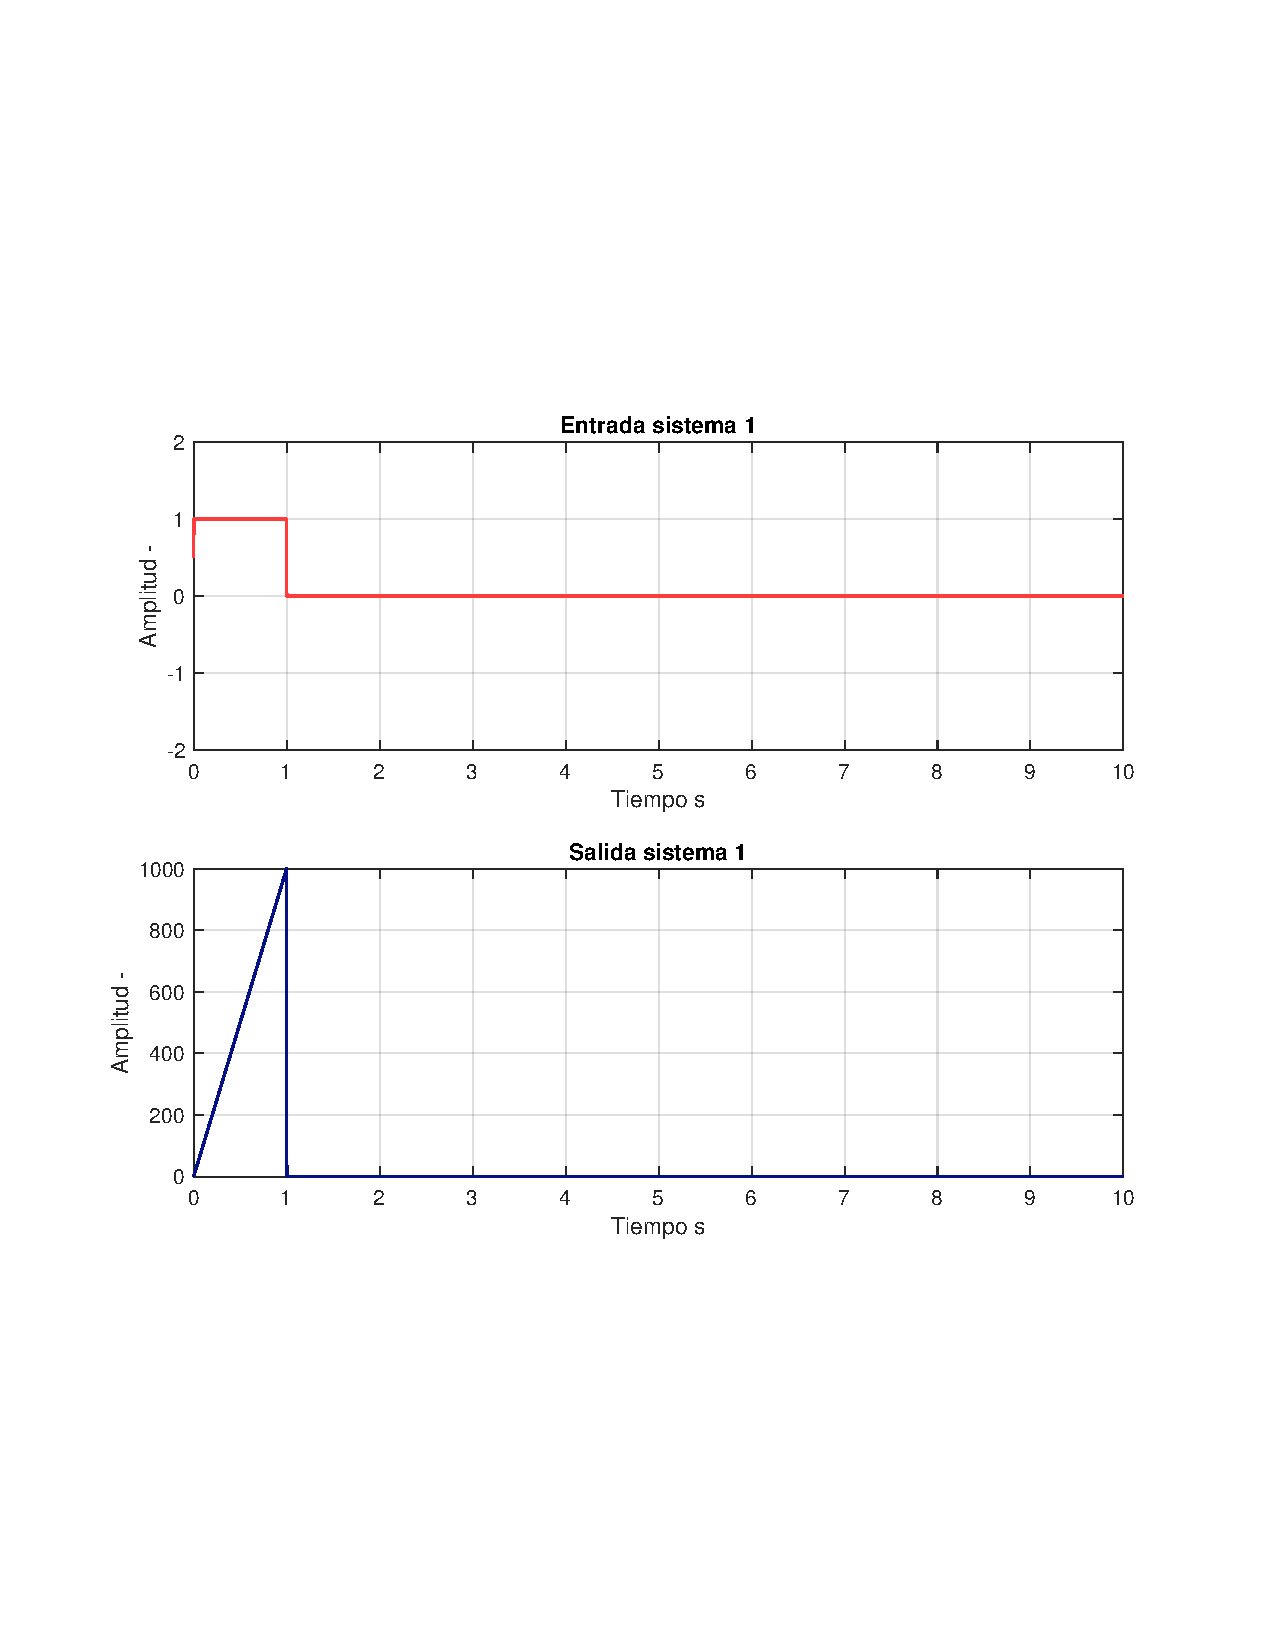
\includegraphics[width=0.6\textwidth,clip, trim = {2cm 7.0cm 2.2cm 7.0cm}]{../imgs/sistema_1_invarianza_temporal_noretardo.pdf}
				\caption{Sistema \#1 Entrada: Pulso cuadrado, de duración 1 \textit{s} \textbf{(Arriba)}. Salida del sistema \textbf{(Abajo)}.}
				\label{fig:s_1_time_invariant_test_1}
			\end{figure}
			
			Generando un retardo para la señal de entrada, equivalente a 5 \textit{s}, se obtiene:
			
			\begin{figure}[H]
				\center
				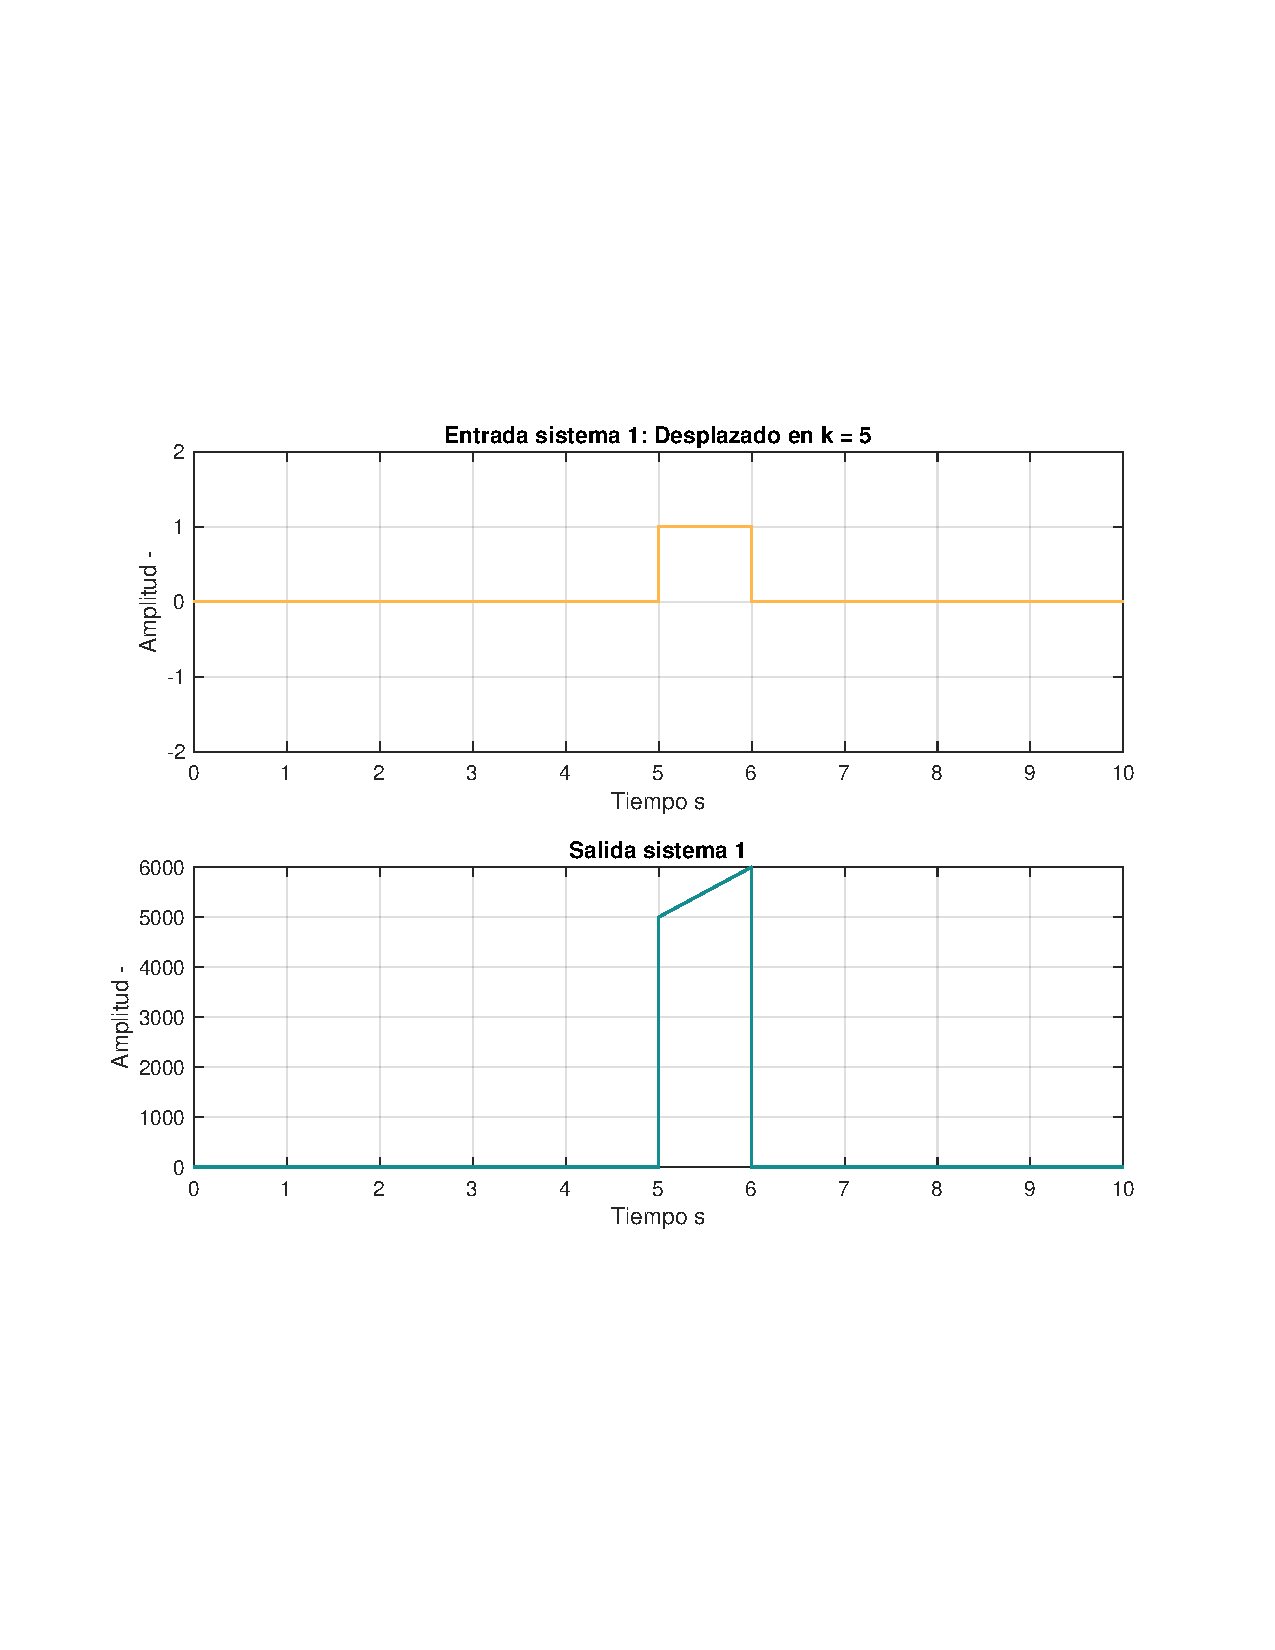
\includegraphics[width=0.6\textwidth,clip, trim = {2cm 7.0cm 2.2cm 7.0cm}]{../imgs/sistema_1_invarianza_temporal_retardo.pdf}
				\caption{Sistema \#1 Entrada: Pulso cuadrado de duración 1 \textit{s}, con un retardo de 5 \textit{s} \textbf{Arriba}.Salida del sistema \textbf{Abajo}.}
				\label{fig:s_1_time_invariant_test_2}
			\end{figure}
			
			A partir de los resultados, claramente el sistema es \textbf{variante en el tiempo}, dado que la señal de entrada retardada no equivale a la señal de salida retardada, no cumpliendo la definición de un sistema invariante según ecuación \ref{eq:cond_invarianza_temporal}.

\newpage

		\subsubsection{Linealidad}
			Se generaron las entradas del sistema, $u_{1}[n]$ y $u_{2}[n]$: 
			\begin{figure}[H]
				\center
				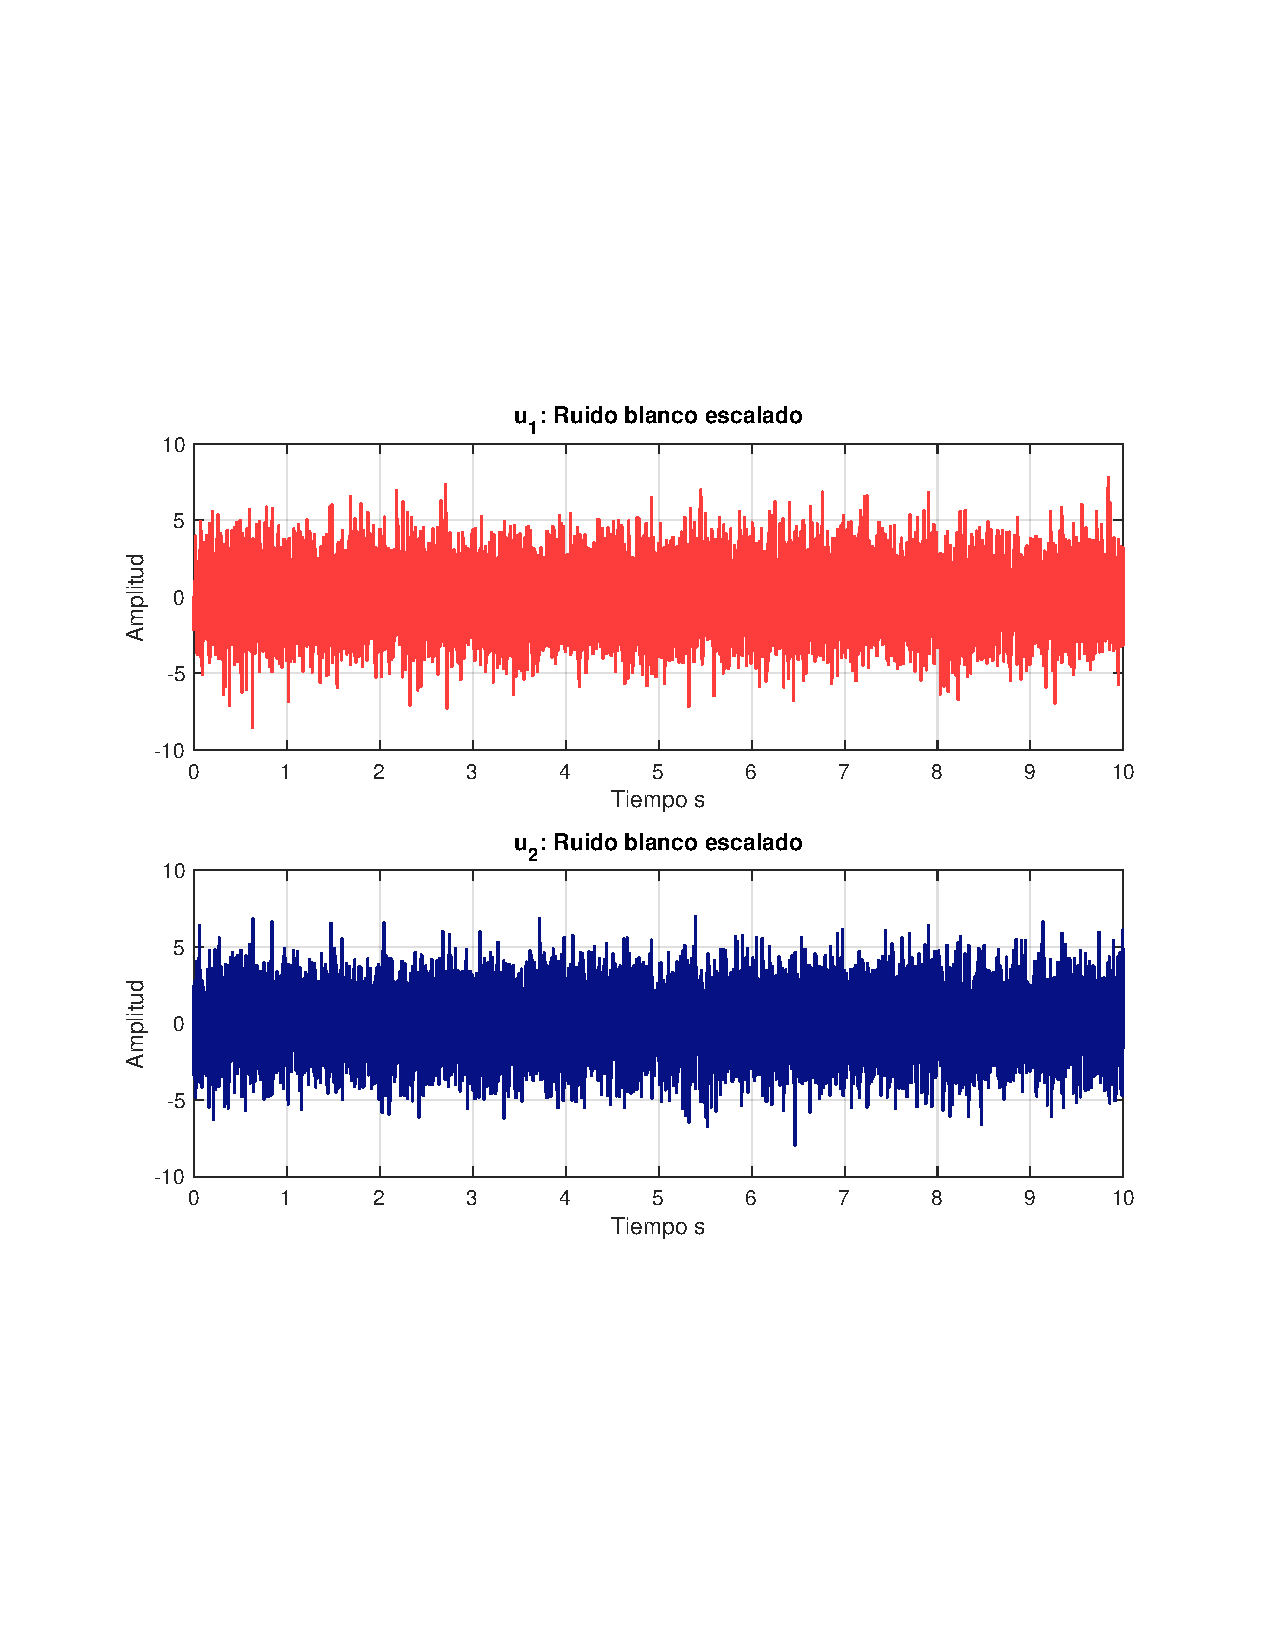
\includegraphics[width=0.6\textwidth,clip, trim = {2cm 7.0cm 2.2cm 7.0cm}]{../imgs/sistema_1_linealidad_entradas.pdf}
				\caption{Entradas del sistema}
				\label{fig:s_1_lineality_inputs}
			\end{figure}

			Para comprobar la linealidad, se necesita que la ecuación \ref{eq:cond_linealidad} se cumpla tanto a su lado izquierdo como derecho, por lo que se genero los términos correspondientes a ambos lados, utilizando la notación dada por la expresión \ref{eq:lineality_outputs}:
			
			\begin{figure}[H]
				\center
				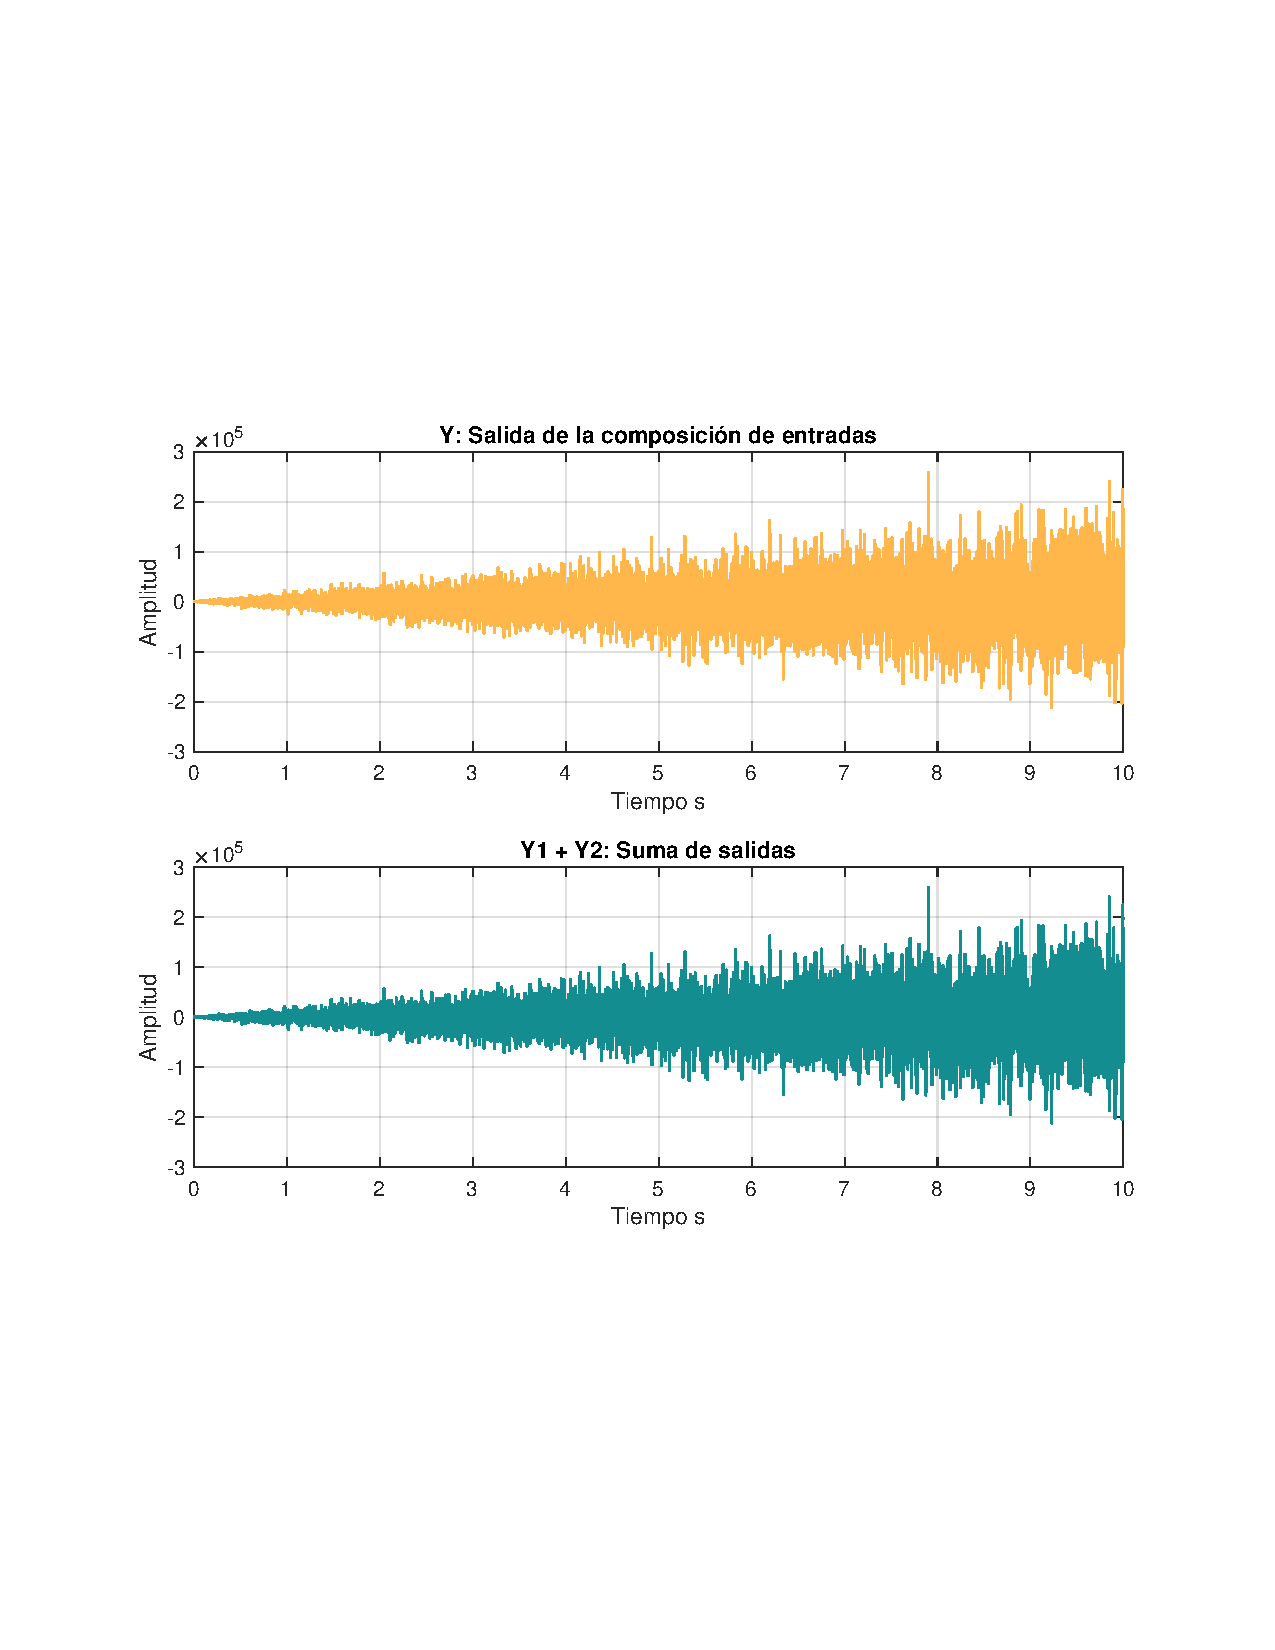
\includegraphics[width=0.6\textwidth,clip, trim = {2cm 7.0cm 2.2cm 7.0cm}]{../imgs/sistema_1_linealidad_salidas.pdf}
				\caption{Salidas del sistema: $Y[n]$ \textbf{(Arriba)}. $Y_{1}[n] + Y_{2}[n]$ \textbf{(Abajo)}.}
				\label{fig:s_1_lineality_outputs}
			\end{figure}
			
			A simple vista, se puede especular que el sistema se comporta de manera lineal, para comprobar esta aseveración, se superpondrá una señal sobre la otra y se calculará la diferencia entre ambas:
			\begin{figure}[H]
				\center
				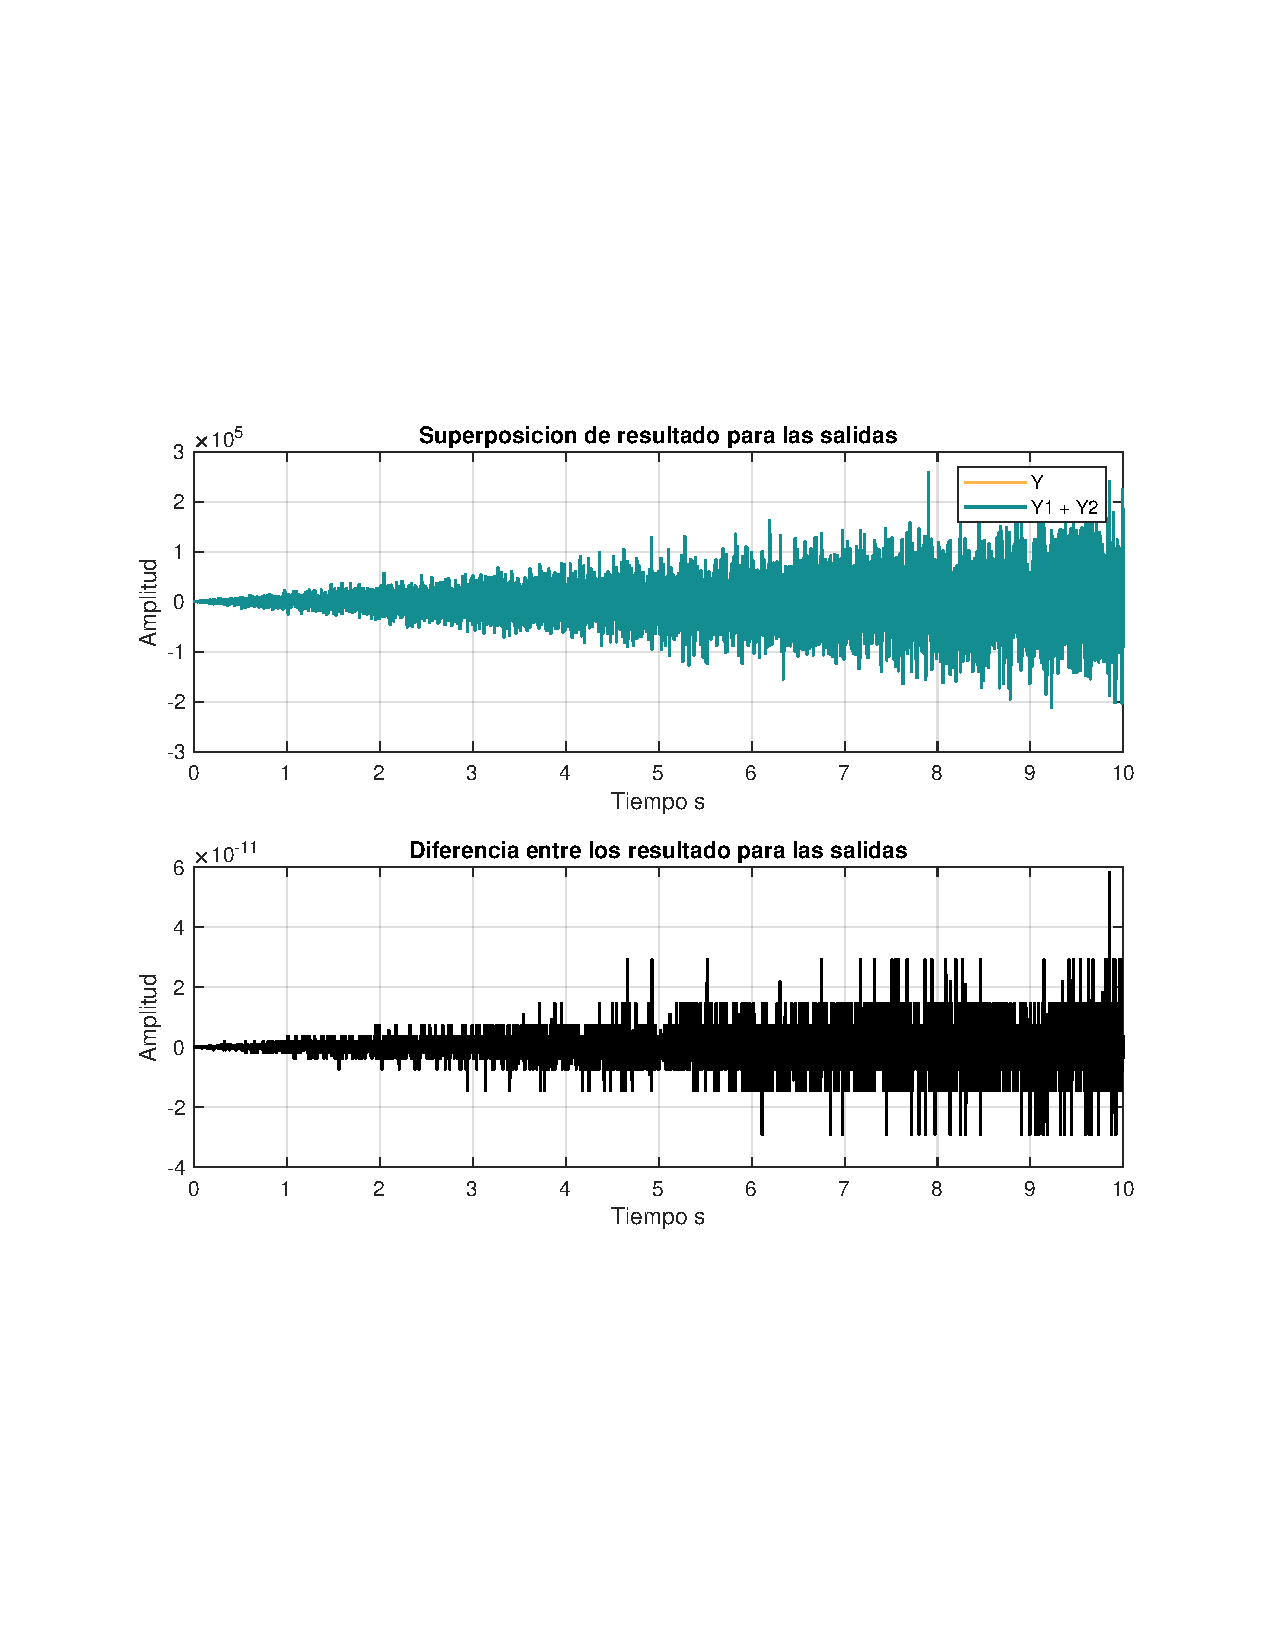
\includegraphics[width=0.6\textwidth,clip, trim = {2cm 7.0cm 2.2cm 7.0cm}]{../imgs/sistema_1_linealidad_superpuestas.pdf}
				\caption{Superposición de las señales de salida \textbf{(Arriba)}. Representación de la resta punto a punto de las señales. \textbf{(Abajo)}.}
				\label{fig:s_1_lineality_superposition}
			\end{figure}
			
			Como se puede observar en la parte superior de la Figura \ref{fig:s_1_lineality_superposition}, ambas señales son iguales, lo que se puede comprobar en la parte inferior de la misma figura, que representa la diferencia:
			\begin{equation*}
				Y [n] -  \left( Y_{1} [n] + Y_{2}[n] \right) 
			\end{equation*}
			
			Dado, que esta está en el orden de $10^{-11}$ se puede concluir que ambas señales son iguales, por lo tanto el sistema es \textbf{lineal}.\footnote{Esta diferencia se puede atribuir a redondeos en tiempo de ejecución realizados por el programa al evaluar las entradas en el sistema}
			
		\subsubsection{Estabilidad BIBO}
			Aplicando como señal de entrada, un delta de Kronecker: 
			\begin{figure}[H]
				\center
				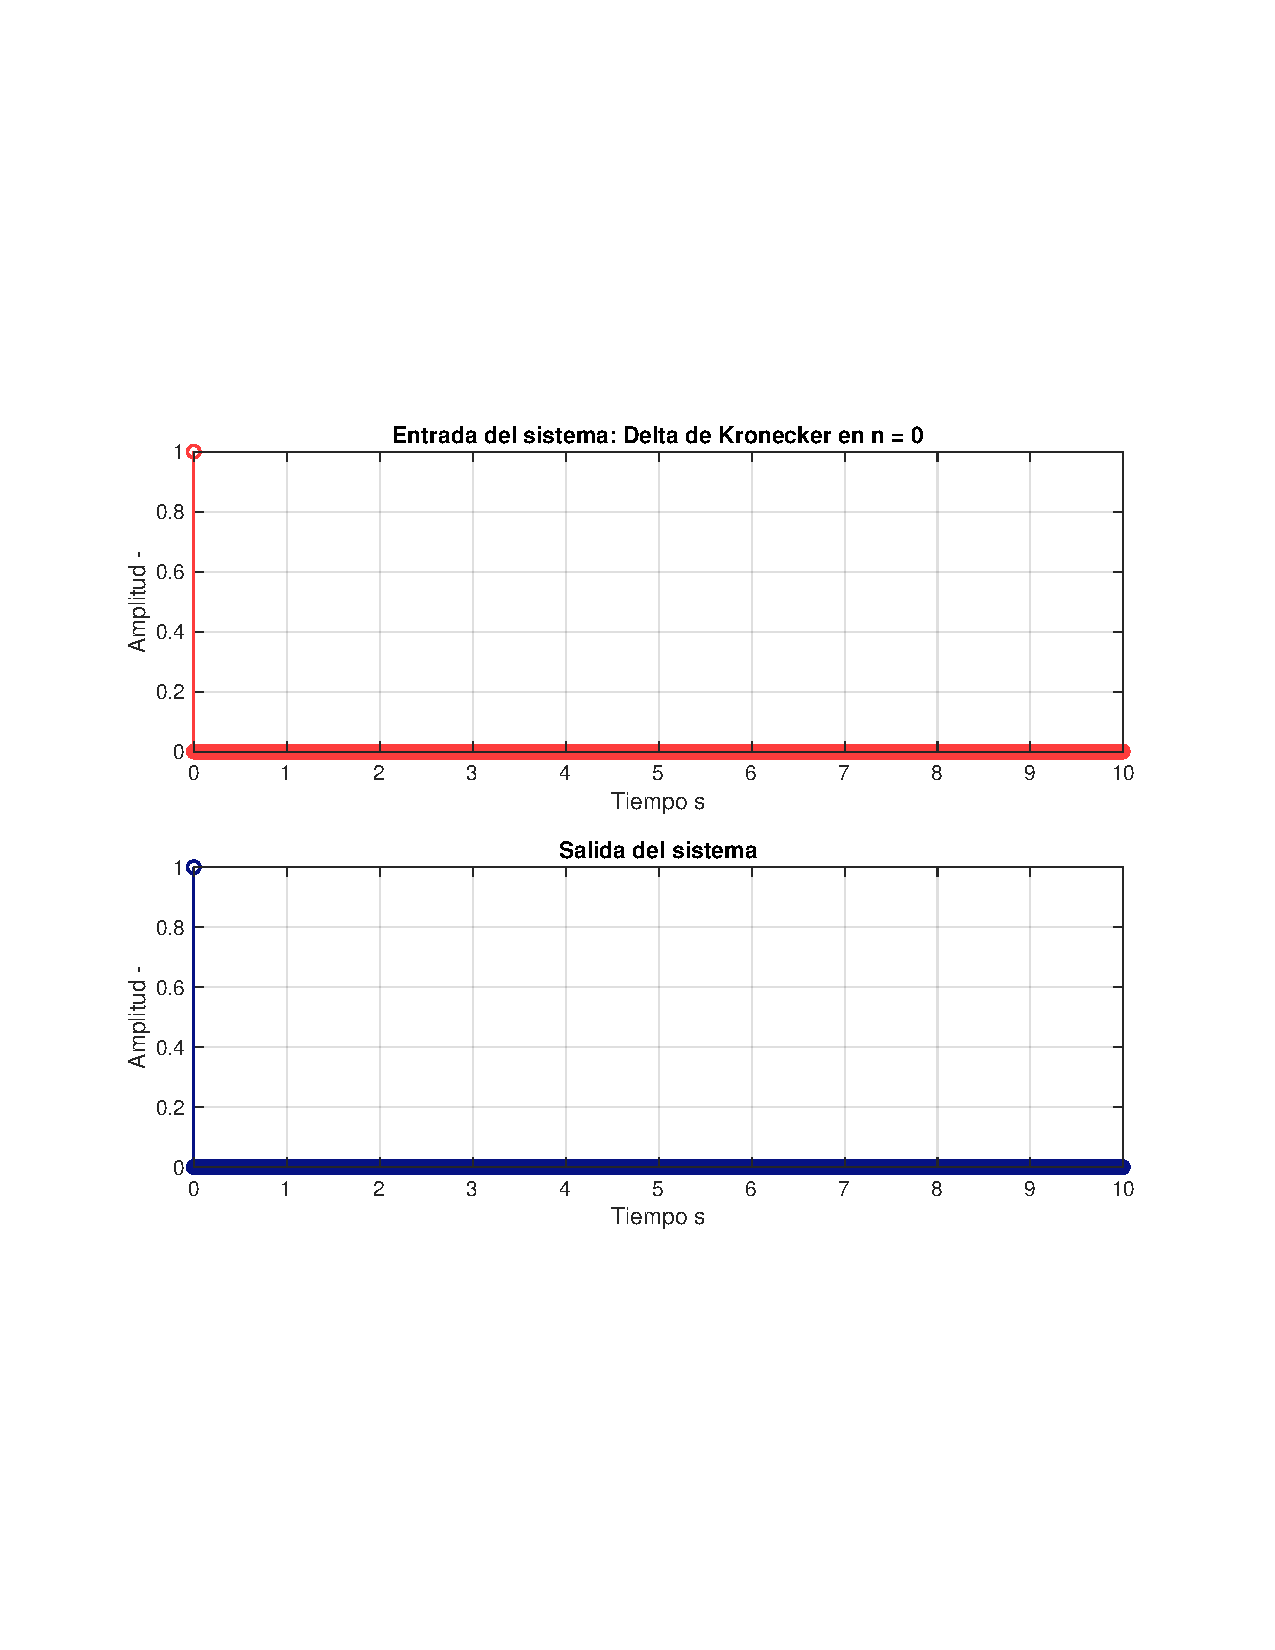
\includegraphics[width=0.6\textwidth,clip, trim = {2cm 7.0cm 2.2cm 7.0cm}]{../imgs/sistema_1_bibo_n_0.pdf}
				\caption{Sistema \#1, para una entrada de un delta de Kronecker \textbf{(arriba)}, se tiene la siguiente respuesta \textbf{(abajo)}.}
				\label{fig:s_1_bibo_0}
			\end{figure}
			
			Notemos, que el resultado, no es de mucha información dado que considerando únicamente esto, podríamos decir que el sistema se comportaria de forma estable. Sin embargo, modificando la entrada para que ahora tenga un retardo de $n = 50$ muestras:
			\begin{figure}[H]
				\center
				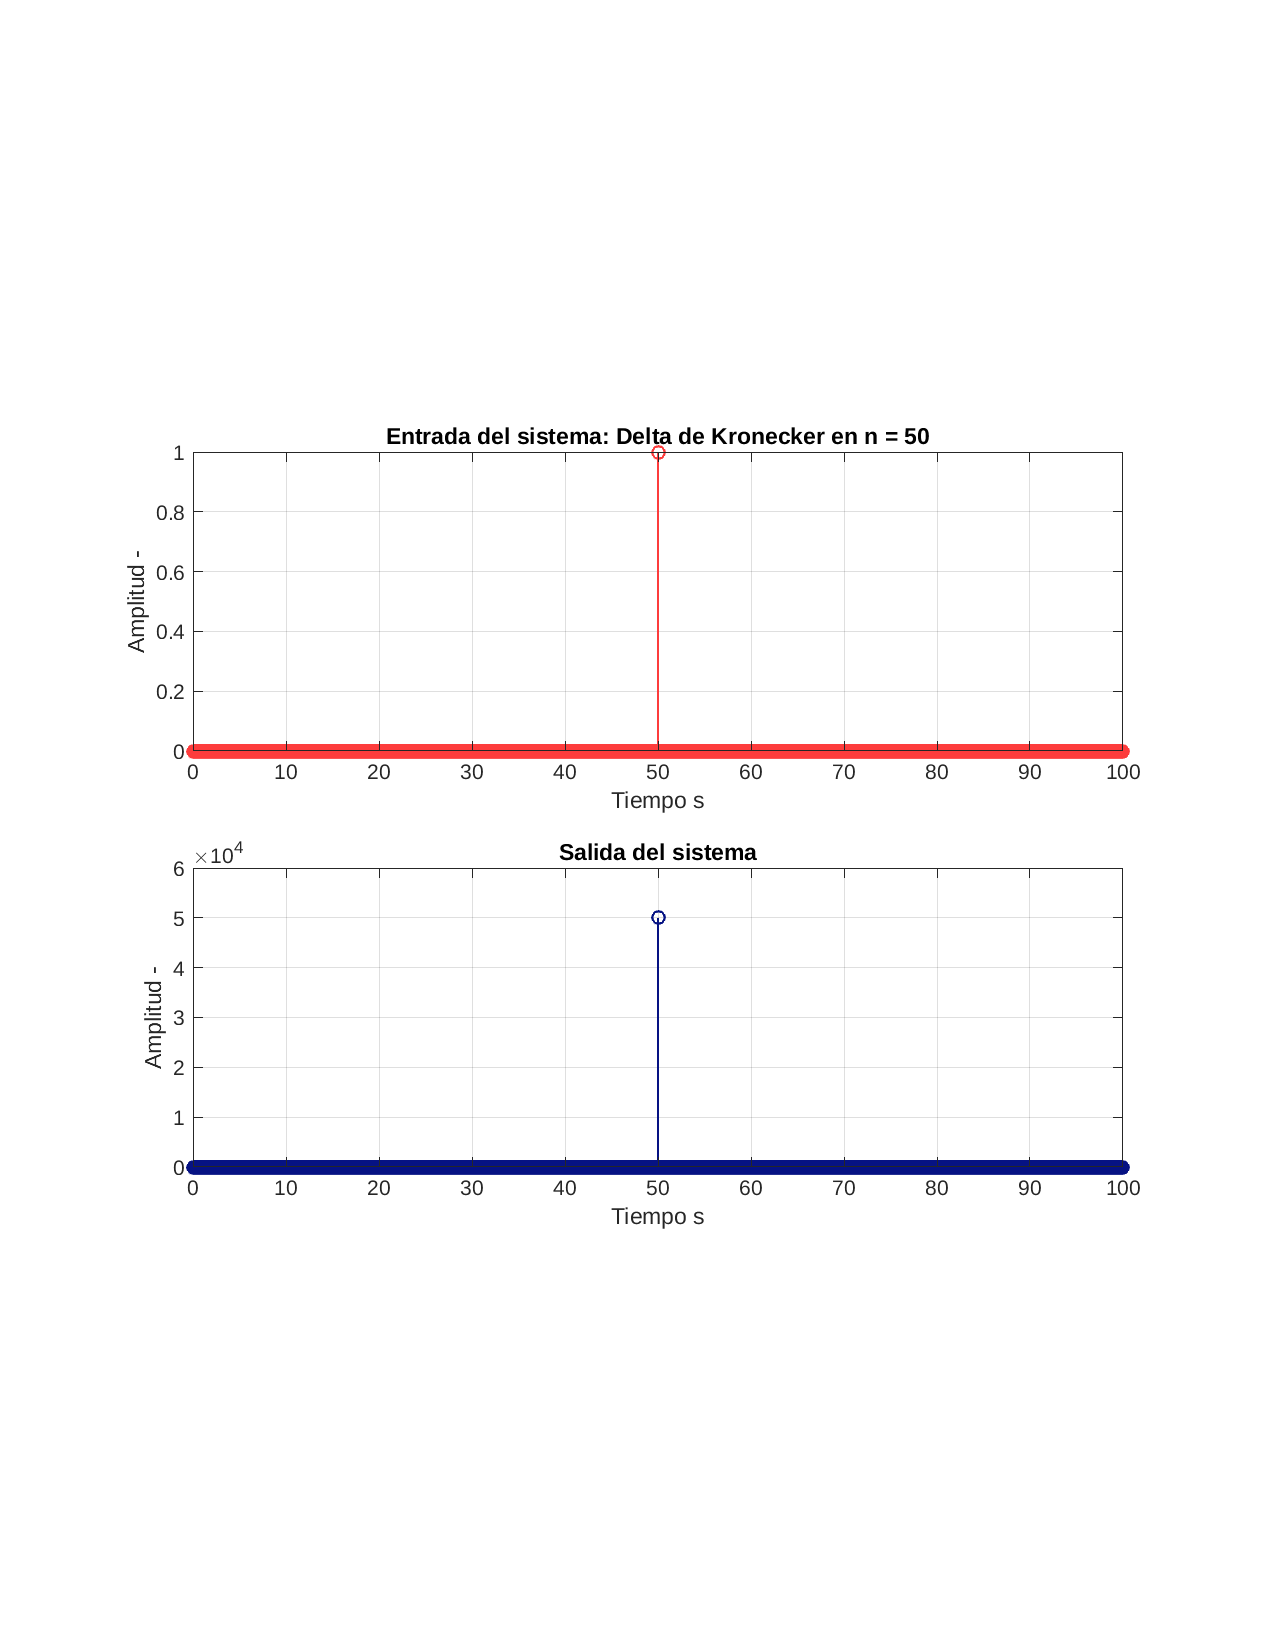
\includegraphics[width=0.6\textwidth,clip, trim = {2cm 7.0cm 2.2cm 7.0cm}]{../imgs/sistema_1_bibo_n_50.pdf}
				\caption{Sistema \#1, para un delta de Kronecker desplazado 50 muestras a la derecha \textbf{(arriba)}. Salida del sistema \textbf{(abajo)}.}
				\label{fig:s_1_bibo_50}
			\end{figure}
			
			Notemos que ahora, se tiene una señal similar a la obtenida en figura \ref{fig:s_1_bibo_0}, sin embargo, ahora el delta que se obtiene a la salida está amplificado por un facotor de ~ $5 \cdot 10^{4}$, esto es debido a que el sistema se comporta como un amplificador, dependiente el tiempo. A medida que avanza el tiempo, la amplificación aumenta:
			\begin{figure}[H]
				\center
				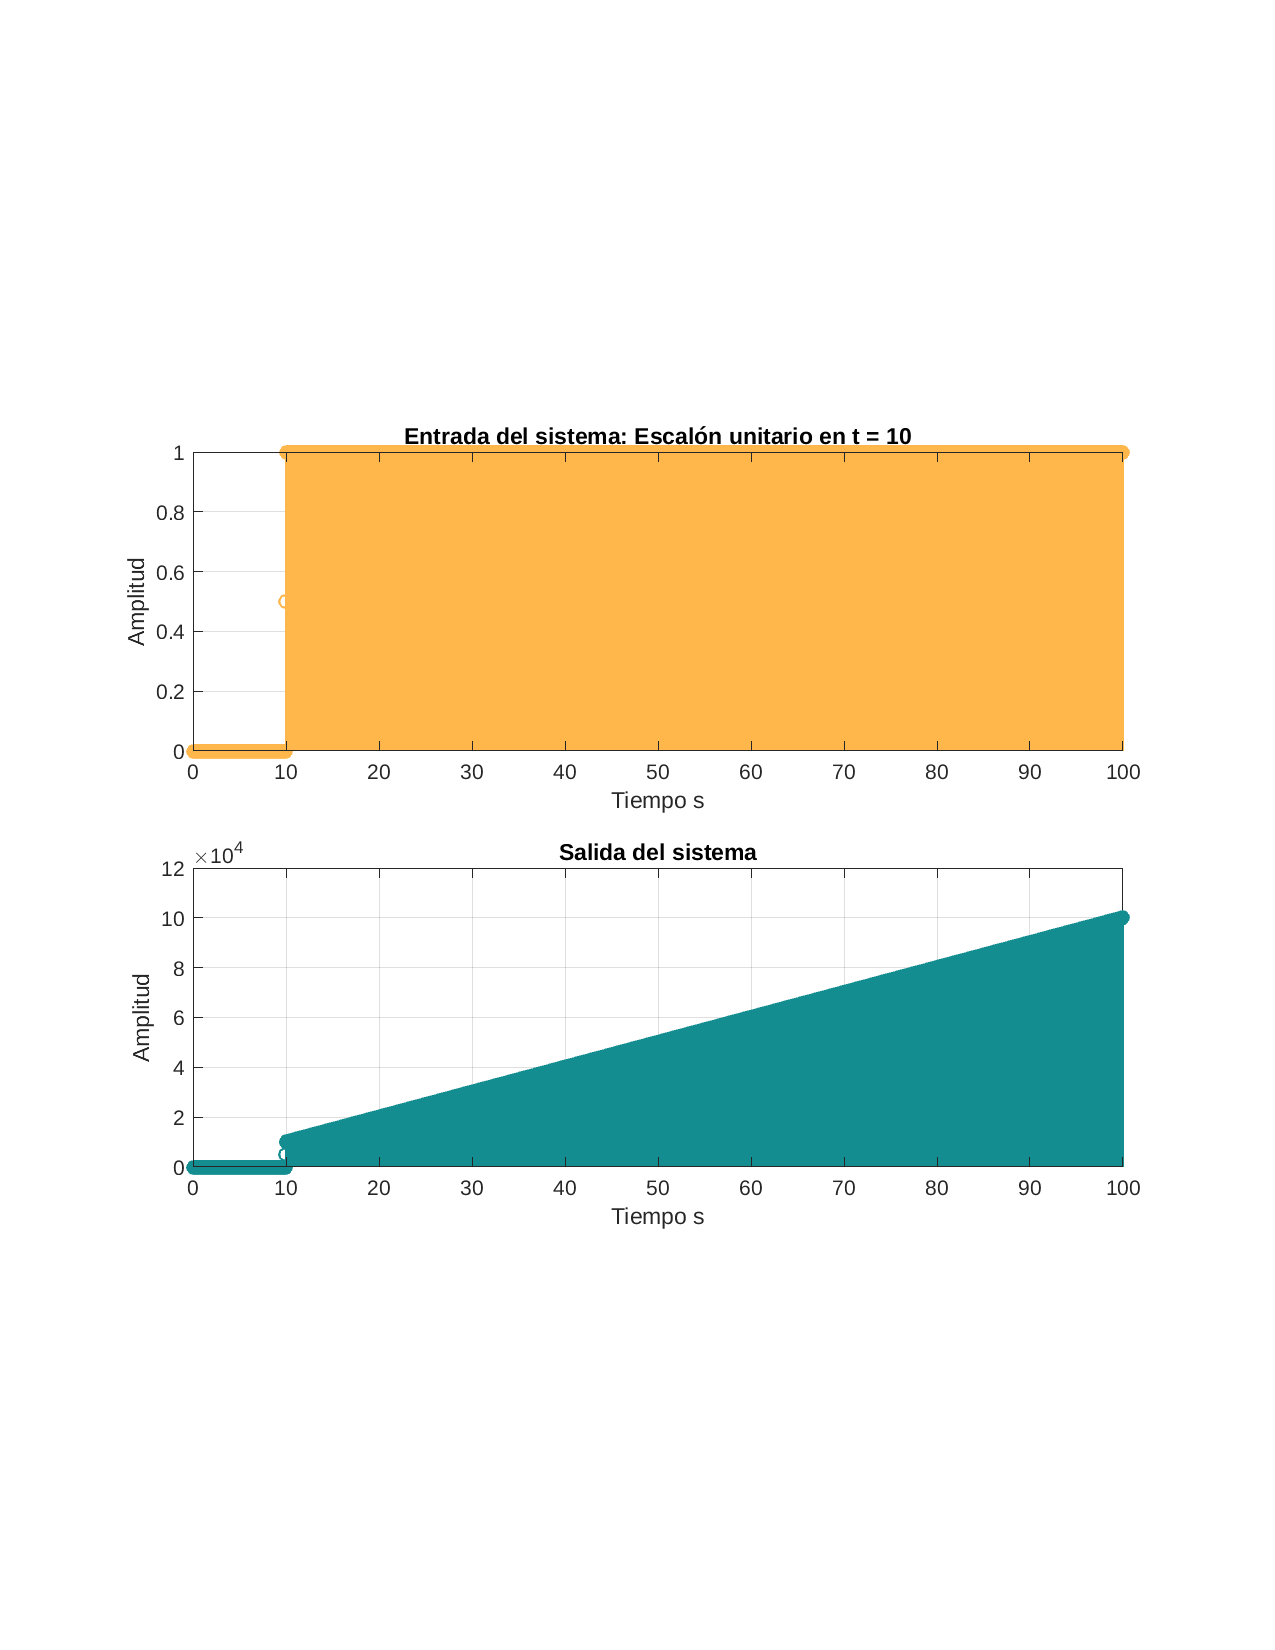
\includegraphics[width=0.6\textwidth,clip, trim = {2cm 7.0cm 2.2cm 7.0cm}]{../imgs/sistema_1_bibo_step.pdf}
				\caption{Sistema \#1, para una escalón unitario, activado en t = 10 \textbf{(arriba)}. Salida del sistema \textbf{(abajo)}.}
				\label{fig:s_1_bibo_step}
			\end{figure}
			
			Como se puede apreciar, a medida que pasa el tiempo, la señal tiende a amplificarse, por lo que se puede especular que si se toma un tiempo muy grande y muestras acorde a este tiempo:
			\begin{equation}
			\lim_{k \rightarrow \infty}  S\{ x[n -k] \} \rightarrow \infty  
			\end{equation}
			
			Dado, que a medida que pasa el tiempo, la amplificación sobre la señal de entrada aumenta, por lo que independiente que $x[n-k]$ sea una señal acotada, la salida del sistema tenderá a infinito. Por lo que podemos especular que el sistema es \textbf{inestable}.\footnote{Note que no es necesario probar con otras señales, dado que ya se comprobó que el sistema es inestable.}
			
\newpage

		\subsection{Sistema \#2}
			\subsubsection{Invariancia temporal}
				Aplicando la señal de prueba en el sistema, con retardo igual a cero:
				\begin{figure}[H]
				\center
				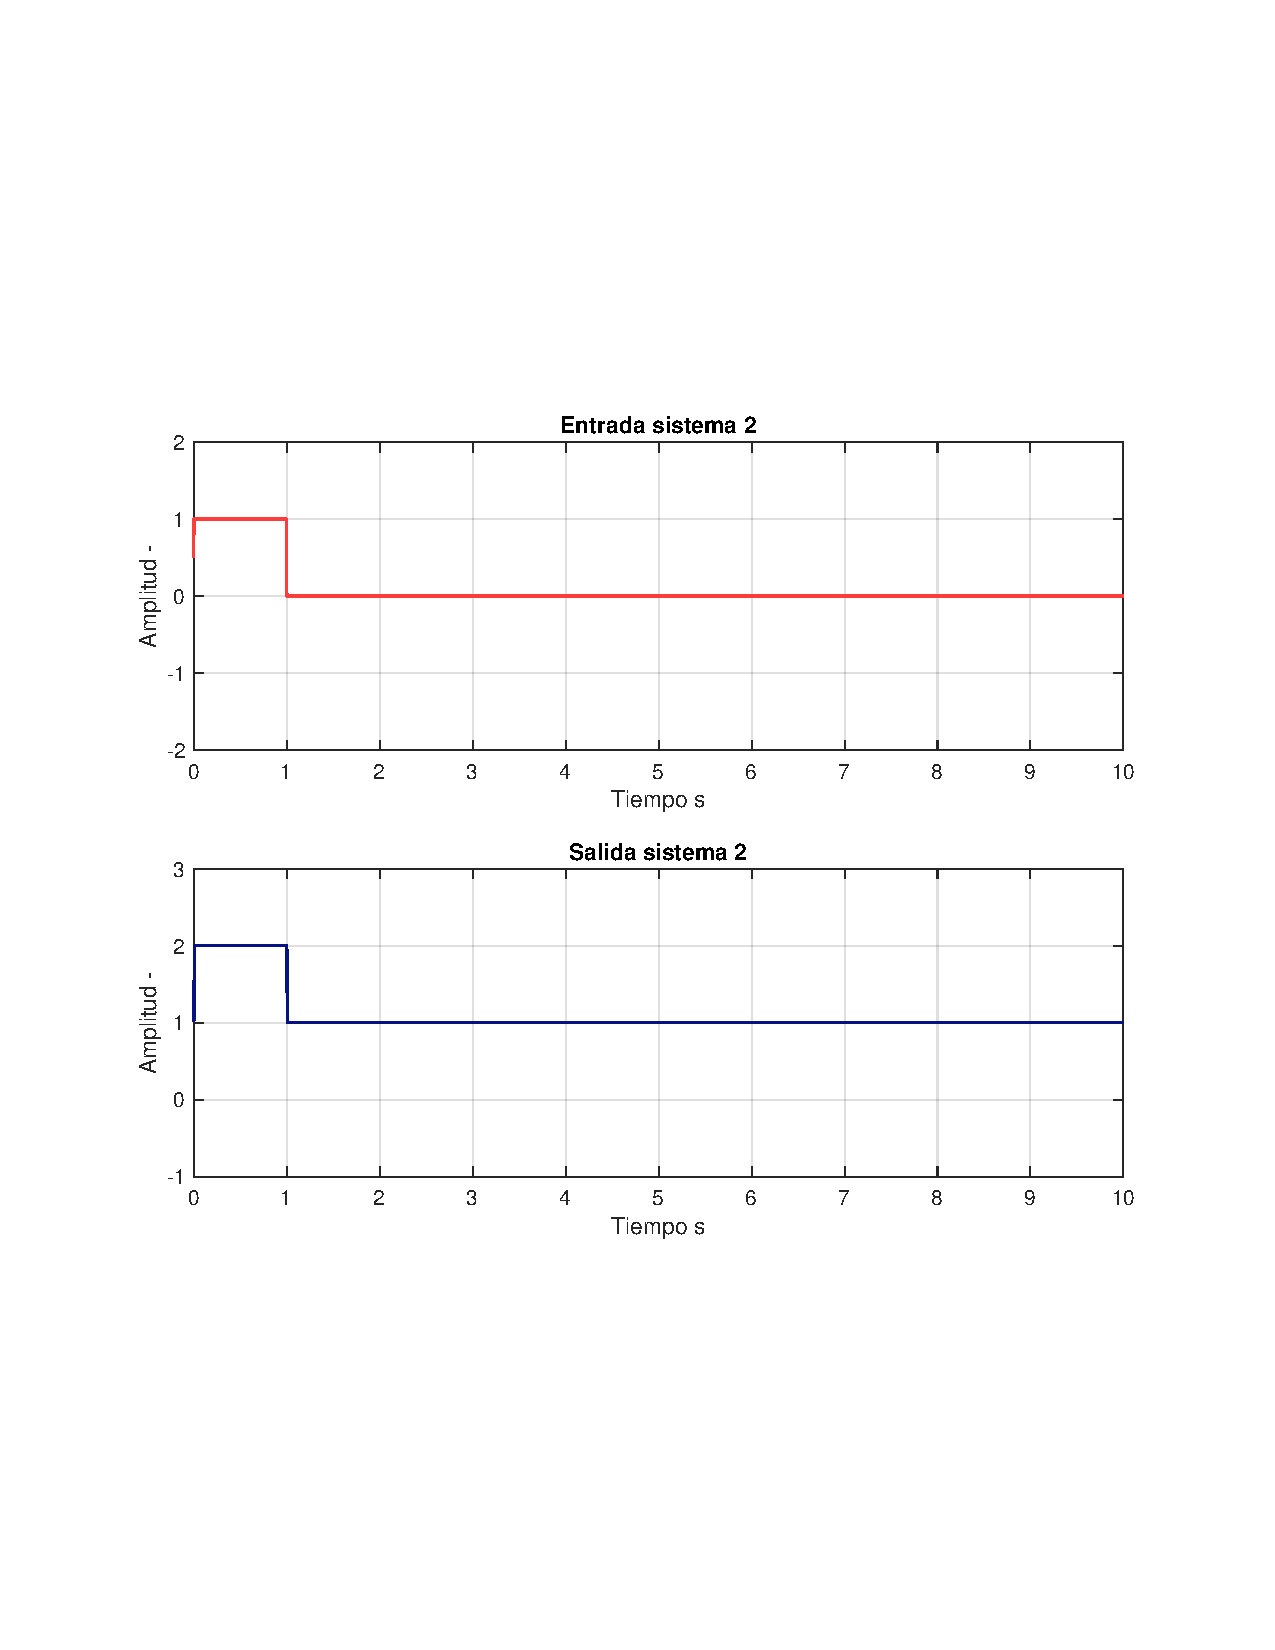
\includegraphics[width=0.6\textwidth,clip, trim = {2cm 7.0cm 2.2cm 7.0cm}]{../imgs/sistema_2_invarianza_temporal_noretardo.pdf}
				\caption{Sistema \#2 Entrada: Pulso cuadrado de duración 1 \textit{s} \textbf{(Arriba)}. Salida del sistema \textbf{(Abajo)}.}
				\label{fig:s_2_time_invariant_test_1}
				\end{figure}
			
				Para un retardo de 5 \textit{s}: 
				\begin{figure}[H]
					\center
					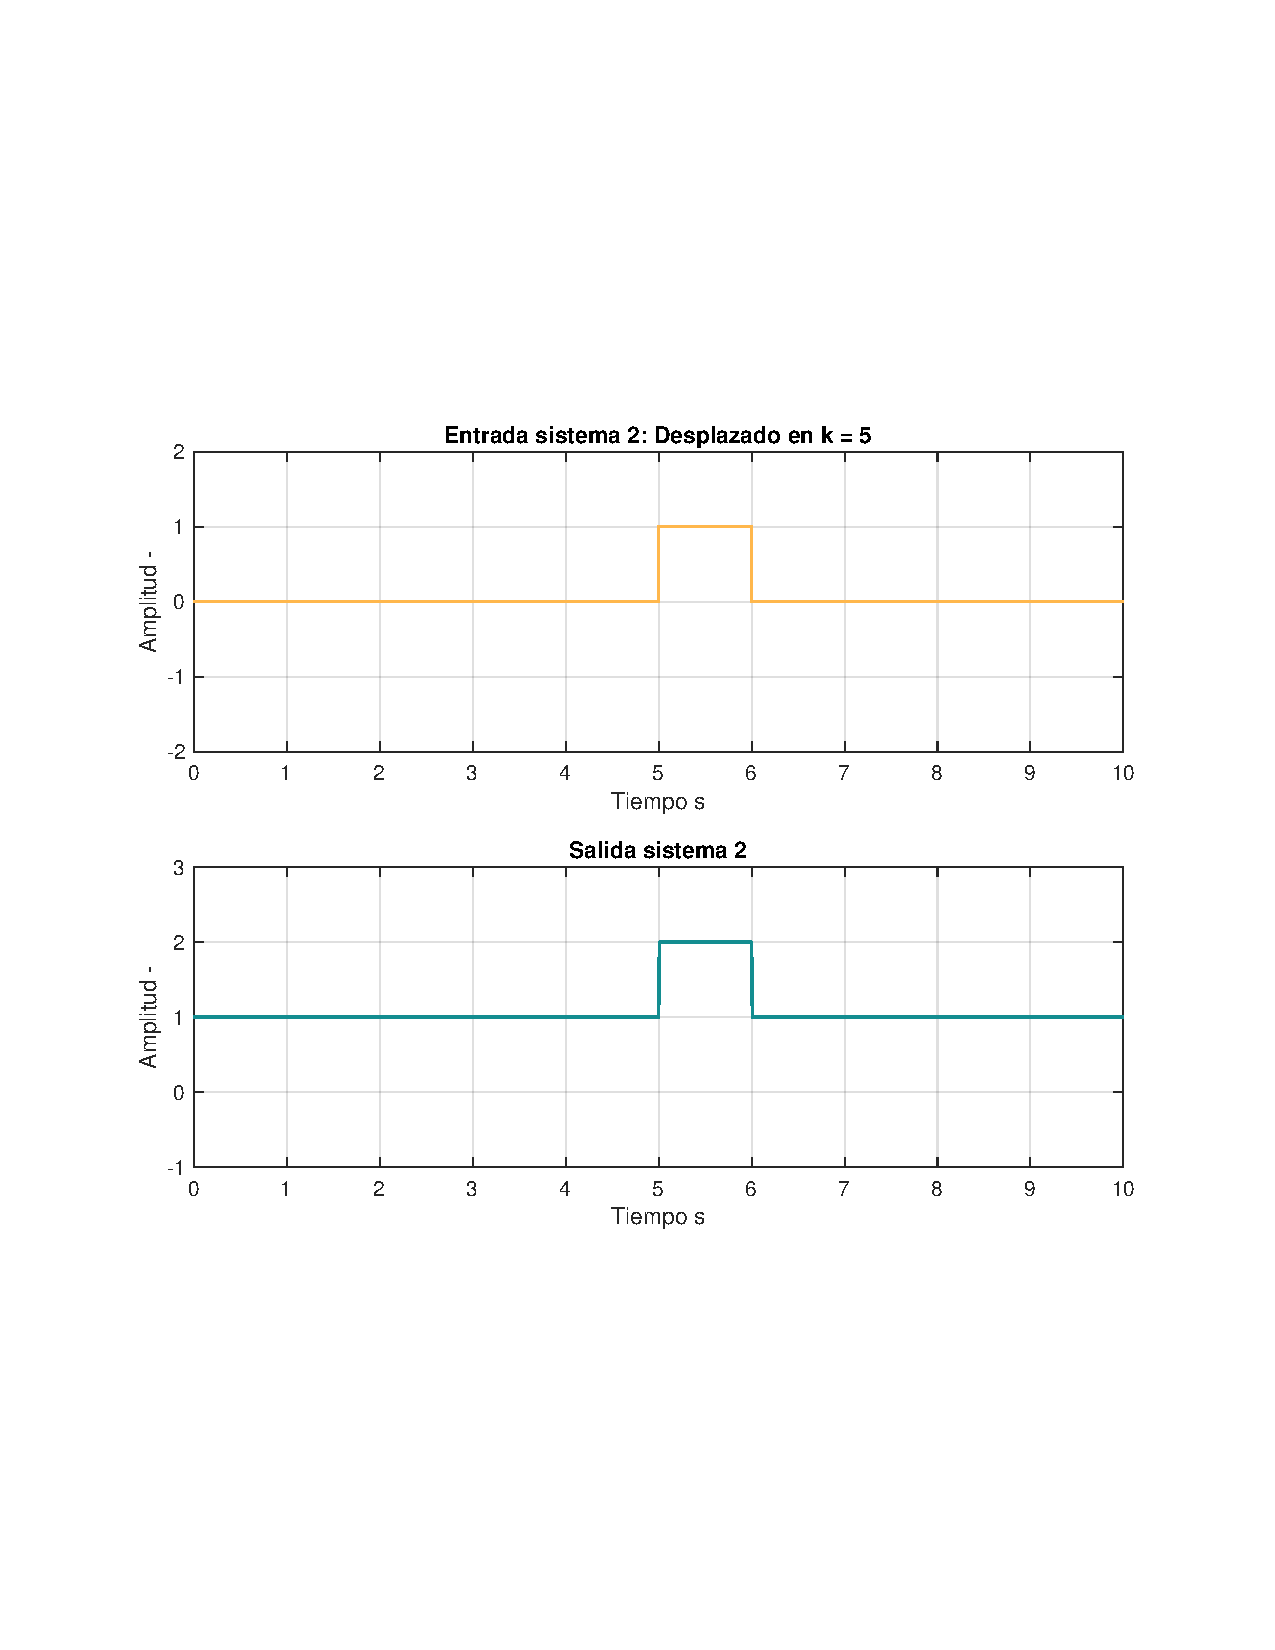
\includegraphics[width=0.6\textwidth,clip, trim = {2cm 7.0cm 2.2cm 7.0cm}]{../imgs/sistema_2_invarianza_temporal_retardo.pdf}
					\caption{Sistema \#2 Entrada: Pulso cuadrado de duración 1 \textit{s}, desplazado en 5 \textit{s} \textbf{(Arriba)}. Salida del sistema \textbf{(Abajo)}.}
					\label{fig:s_2_time_invariant_test_2}
				\end{figure}
			
				Como se ver, al aplicar un retardo sobre la señal de entrada, se obtiene la misma salida sólo que desplazada, cumpliendose la condición descrita en la ecuación \ref{eq:cond_invarianza_temporal}. Por lo que podemos decir que el sistema es \textbf{invariante en el tiempo}. 

\newpage

		\subsubsection{Linealidad}
			Generando las entradas del sistema $u_{1}[n]$ y $u_{2}[n]$:
			\begin{figure}[H]
				\center
				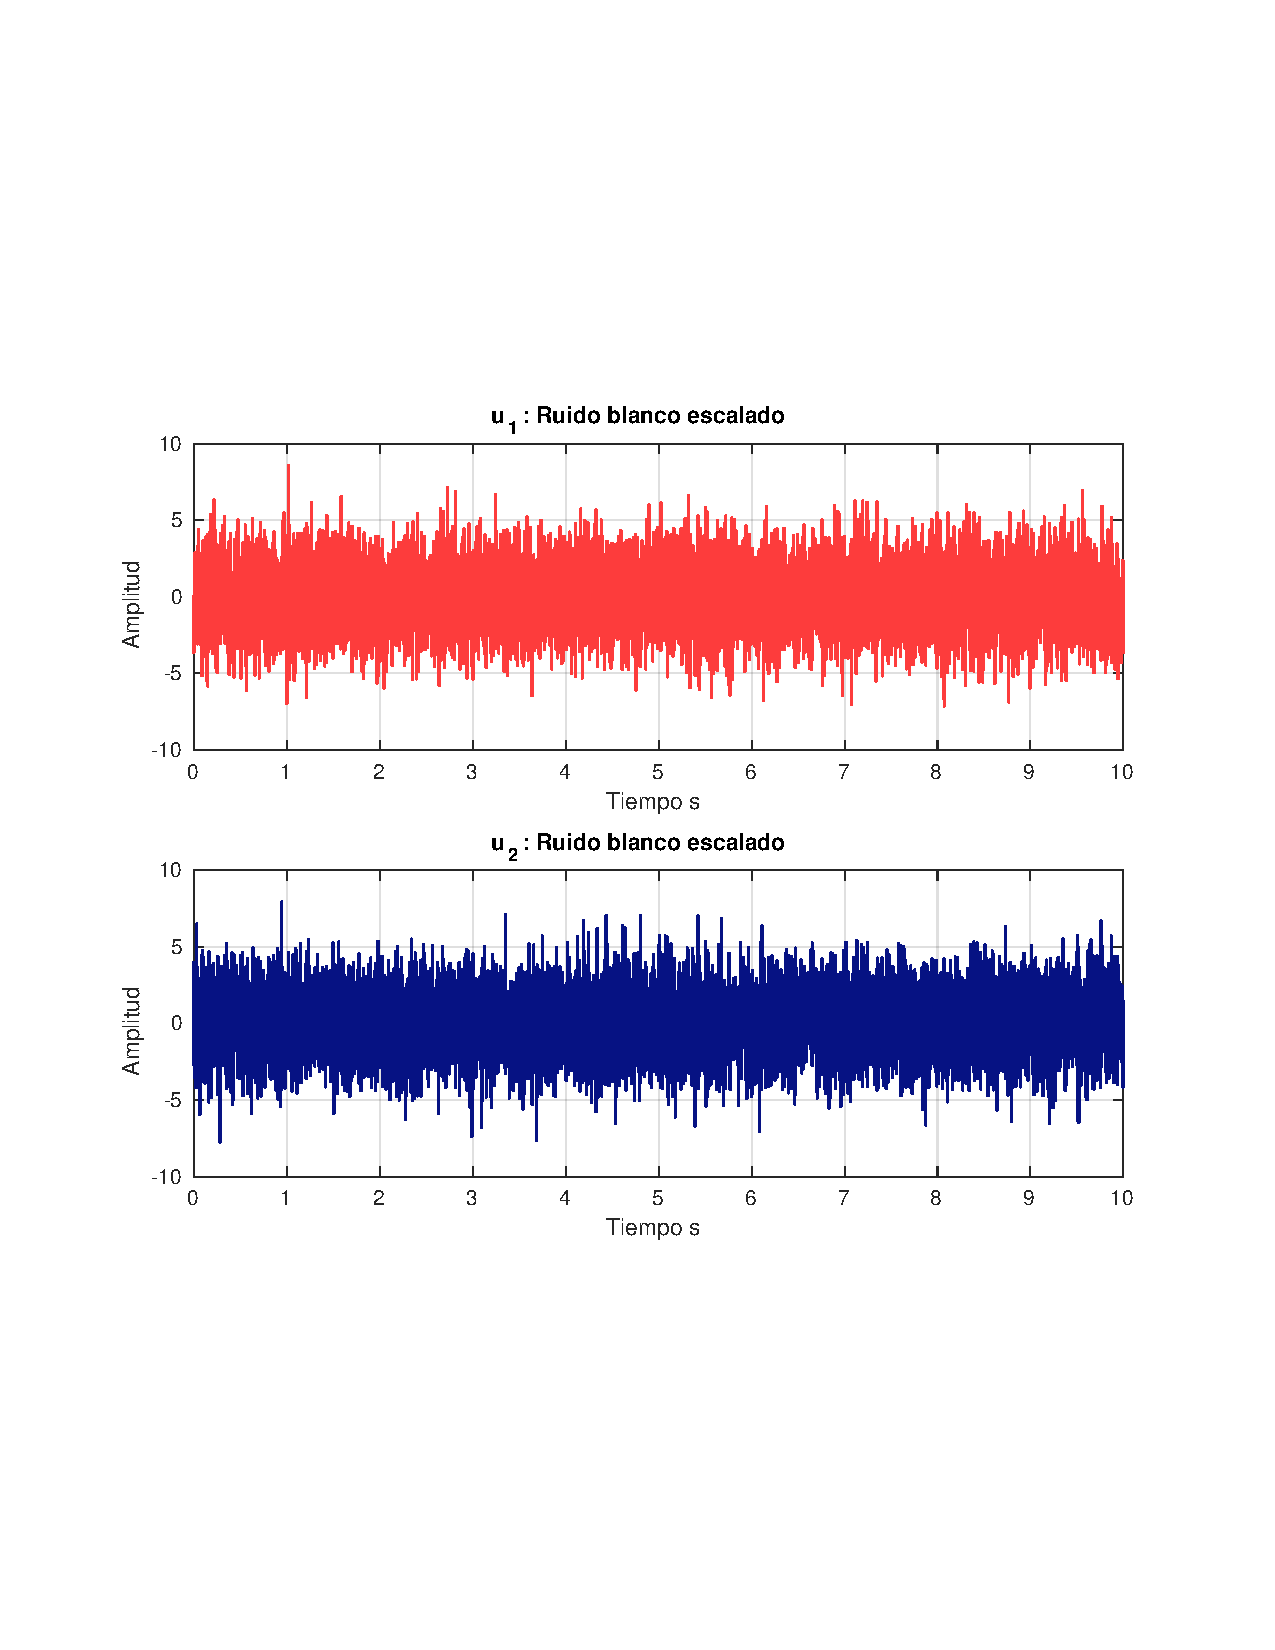
\includegraphics[width=0.6\textwidth,clip, trim = {2cm 7.0cm 2.2cm 7.0cm}]{../imgs/sistema_2_linealidad_entradas.pdf}
				\caption{Entradas del sistema}
				\label{fig:s_2_lineality_inputs}
			\end{figure}
		
			Comprobando las salidas del sistema:
			\begin{figure}[H]
				\center
				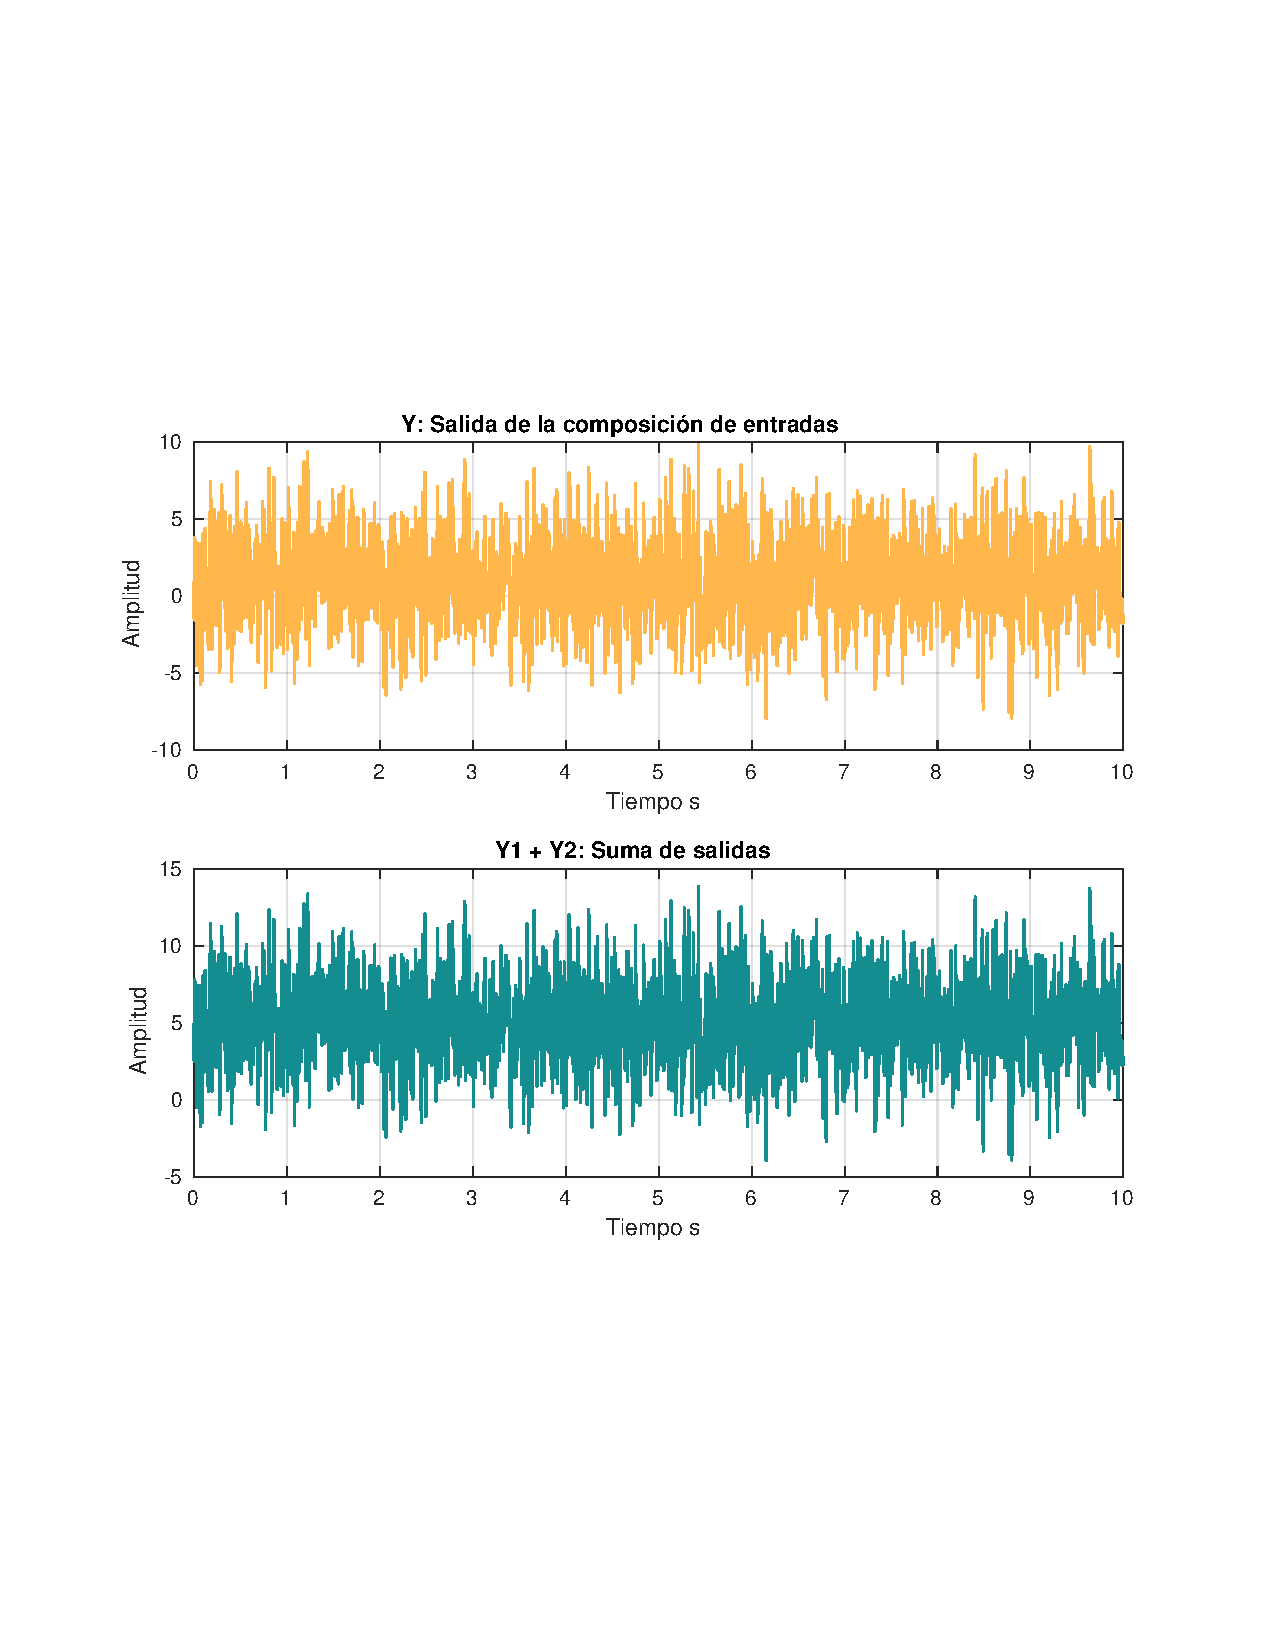
\includegraphics[width=0.6\textwidth,clip, trim = {2cm 7.0cm 2.2cm 7.0cm}]{../imgs/sistema_2_linealidad_salidas.pdf}
				\caption{Salidas del sistema: $Y[n]$ \textbf{(Arriba)}. $Y_{1}[n] + Y_{2}[n]$ \textbf{(Abajo)}.}
				\label{fig:s_2_lineality_outputs}	
			\end{figure}
\newpage
			Realizando la comparación de salidas:
			\begin{figure}[H]
				\center
				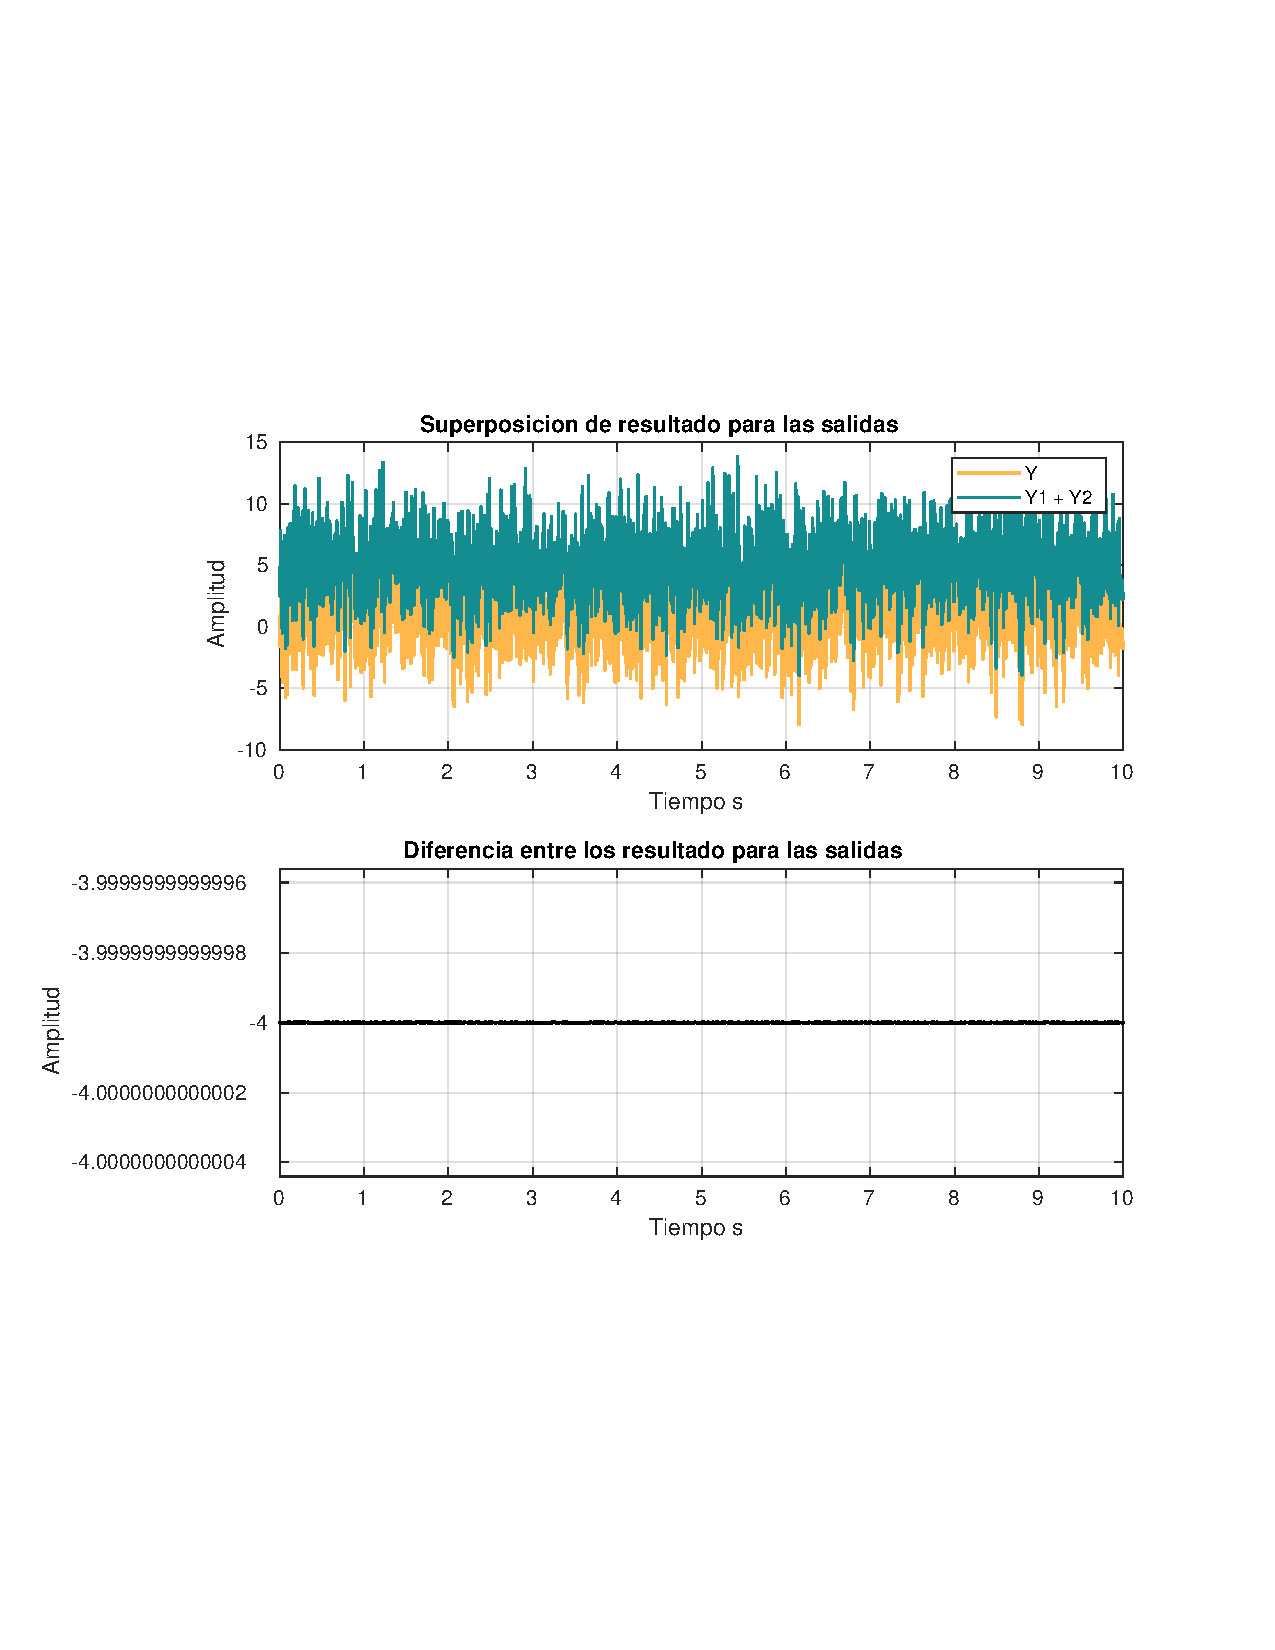
\includegraphics[width=0.6\textwidth,clip, trim = {2cm 7.0cm 2.2cm 7.0cm}]{../imgs/sistema_2_linealidad_superpuestas.pdf}
				\caption{Superposición de las señales de salida \textbf{(Arriba)}. Representación de la resta punto a punto de las señales. \textbf{(Abajo)}.}
				\label{fig:s_2_lineality_superposition}
			\end{figure}
		
			Como se puede ver, en la figura \ref{fig:s_2_lineality_outputs}, ambas salidas son muy similares, sin embargo, la salida que corresponde al resultado del lado derecho de la ecuación \ref{eq:cond_linealidad}, parece faltarle un nivel continuo, lo que queda en evidencia al calcular la diferencia de ambas entradas, figura \ref{fig:s_2_lineality_superposition}. Por lo que podemos concluir que el sistema \textbf{no es lineal}.
		
		\subsubsection{Estabilidad BIBO}
			Aplicandole al sistema un delta de Kronecker:
		
			\begin{figure}[H]
				\center
				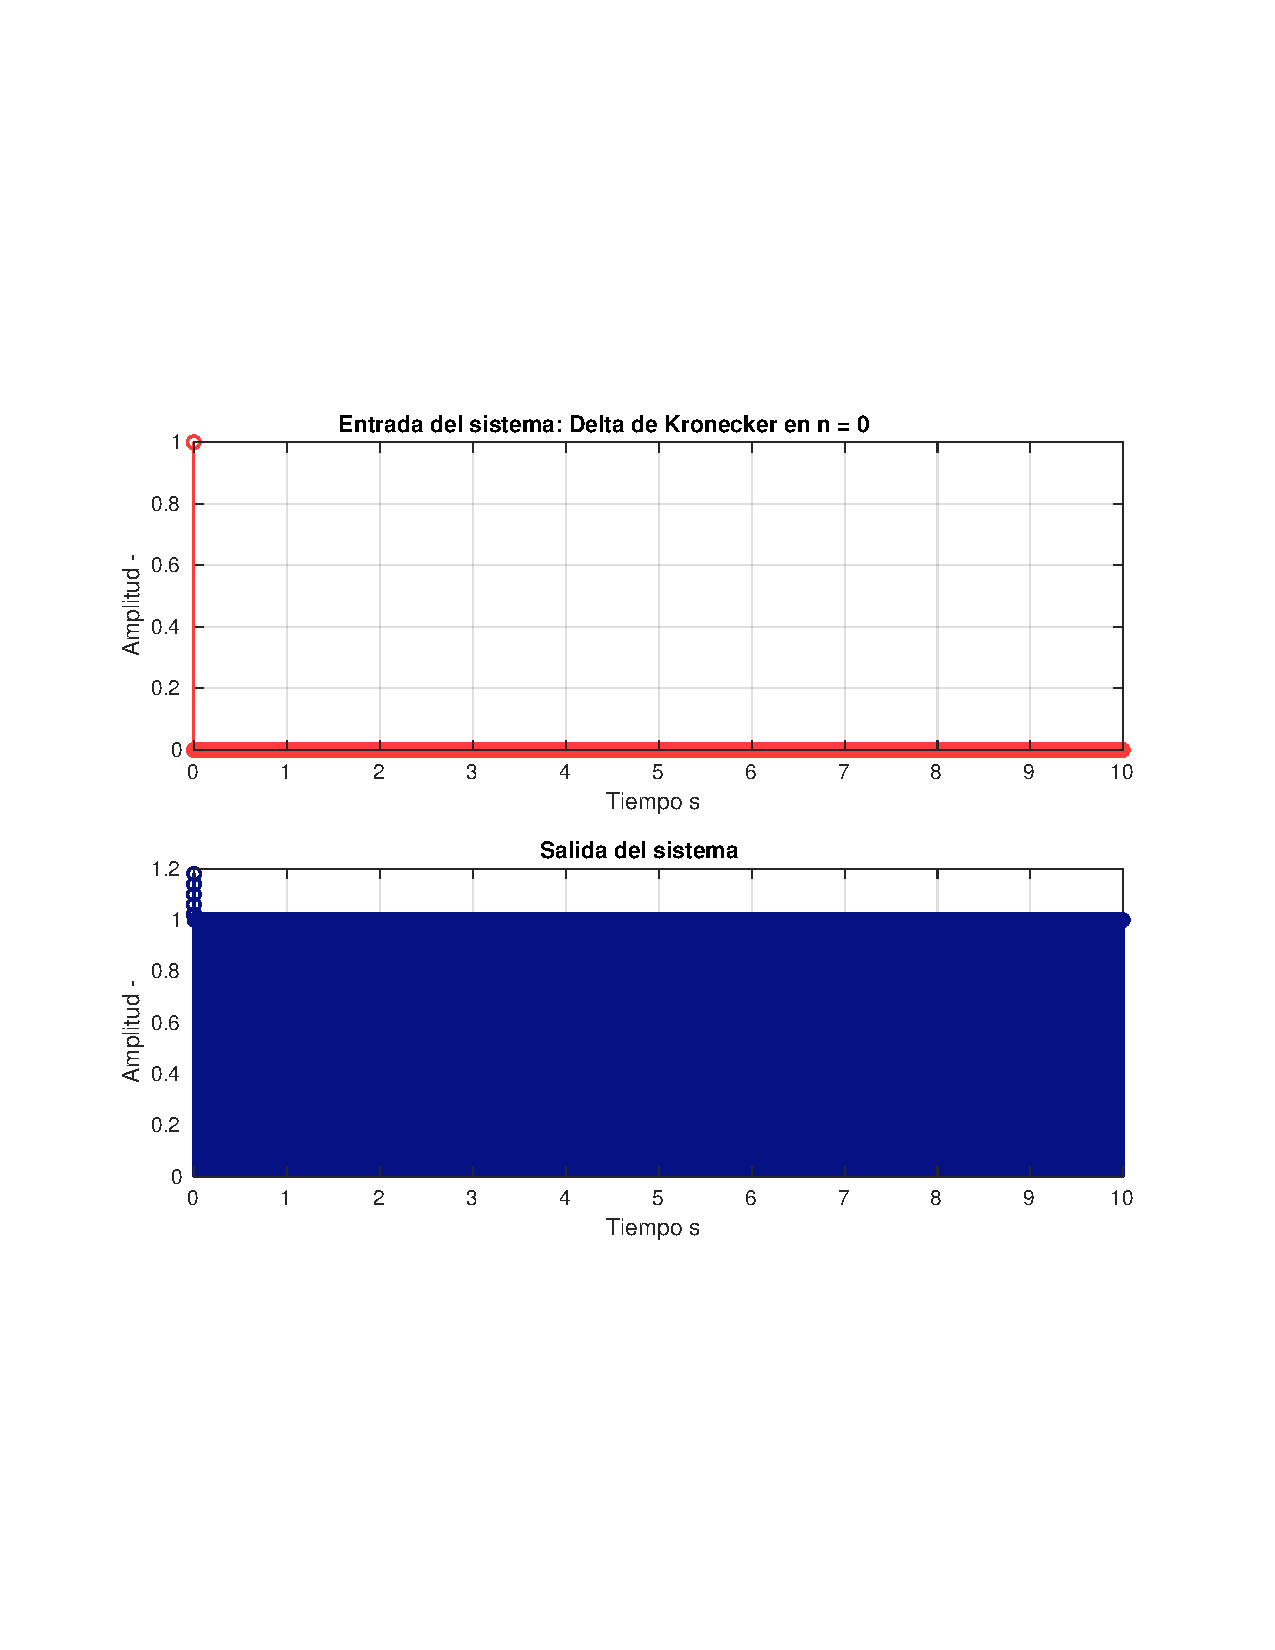
\includegraphics[width=0.6\textwidth,clip, trim = {2cm 7.0cm 2.2cm 7.0cm}]{../imgs/sistema_2_bibo_n_0.pdf}
				\caption{Sistema \#2, para una entrada de un delta de Kronecker \textbf{(Arriba)}, para la cual se tiene la siguiente respuesta \textbf{(Abajo)}.}
				\label{fig:s_2_bibo_n_0}
			\end{figure}
		
			Podemos ver que la salida del sistema, se comporta como la entrada más una constante, algo que ya se había notado durante la comprobación de linealidad del sistema. A partir del resultado, para esta señal, podemos decir que para un delta, el sistema es estable. Procediendo a probar con un escalón unitario:
		
			\begin{figure}[H]
				\center
				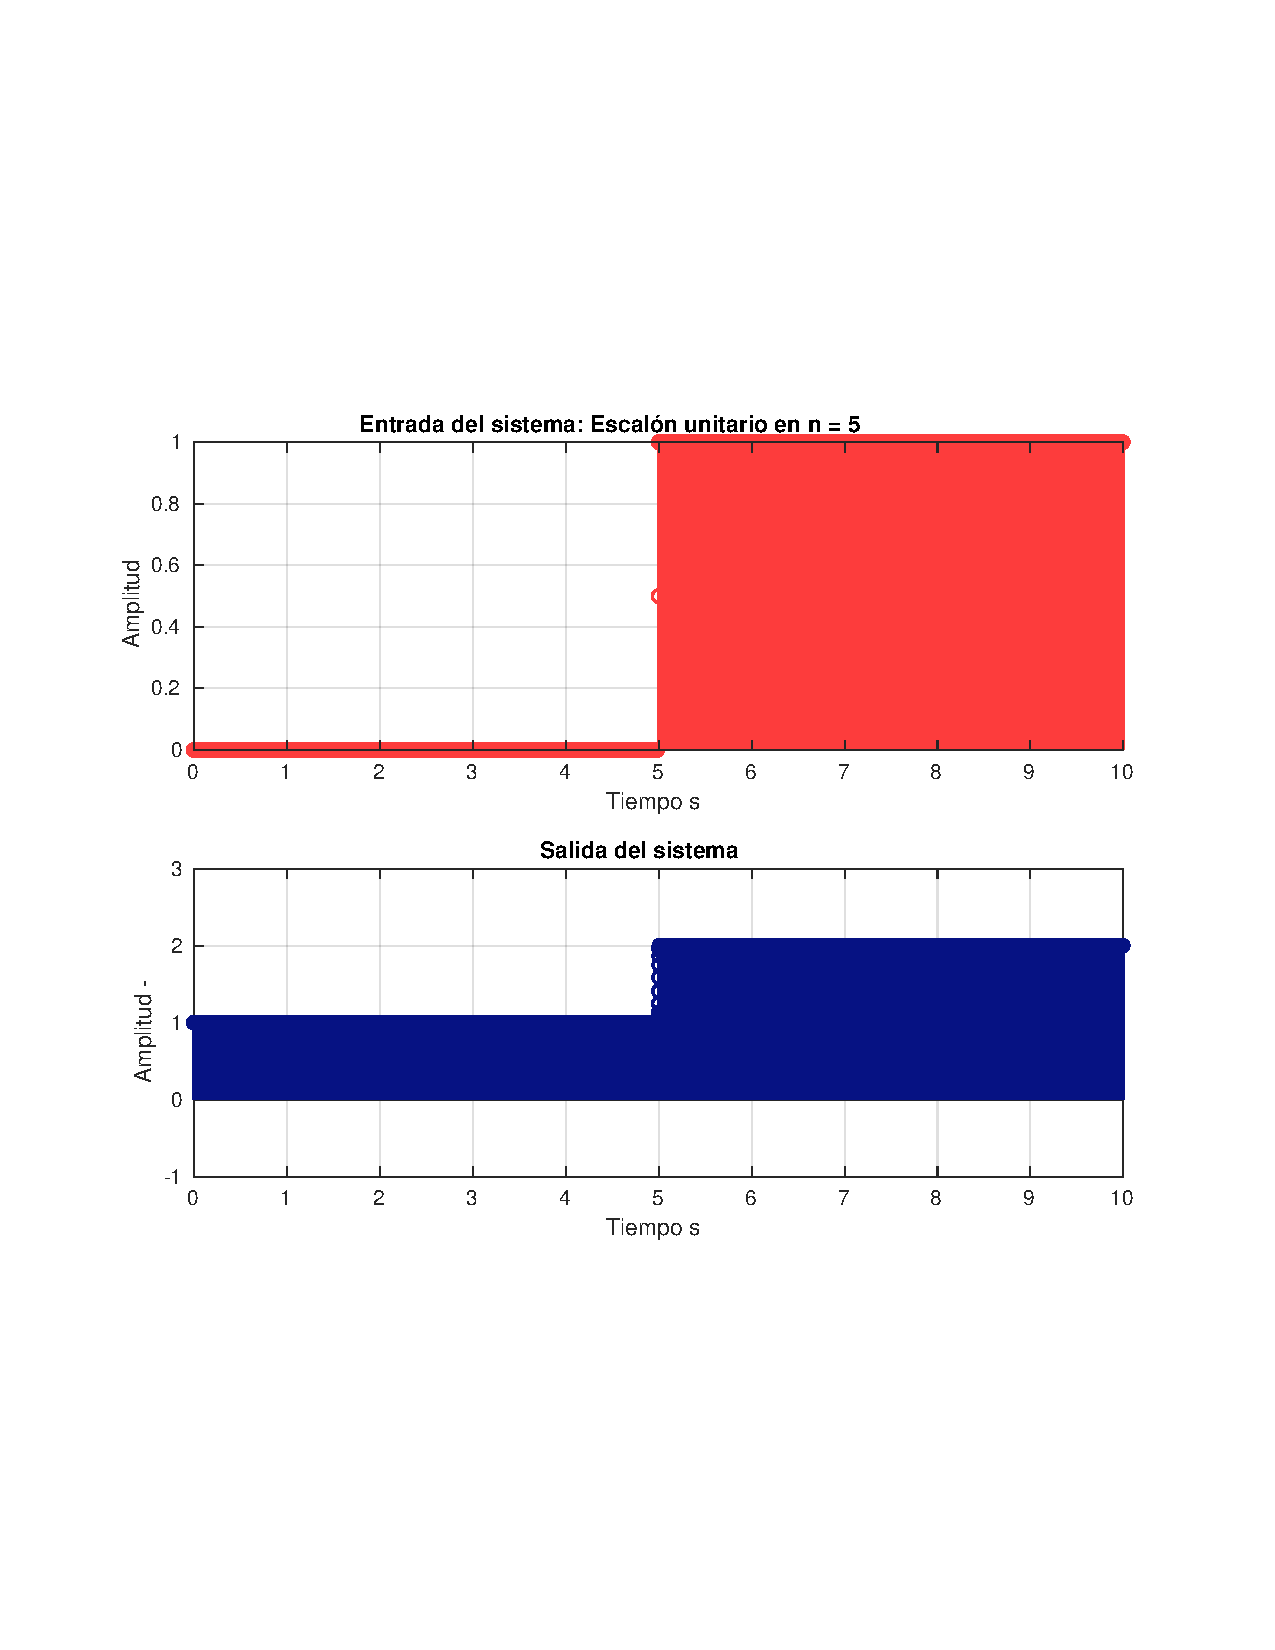
\includegraphics[width=0.6\textwidth,clip, trim = {2cm 7.0cm 2.2cm 7.0cm}]{../imgs/sistema_2_bibo_heaviside_n_5.pdf}
				\caption{Sistema \#2, para una entrada de escalón unitario, activado en n = 5 \textbf{(Arriba}}, para el cual se tiene la siguiente respuesta \textbf{(Abajo)}. 
				\label{fig:s_2_bibo_heaviside_n_5}
			\end{figure}
		
			Para esta salida, también se tiene que el sistema responde sumándole a la entrada una constante. Nuevamente, la respuesta para esta entrada es acotada. Siguiendo con la última señal de prueba, una señal triangular de amplitud 1 y frecuencia 1 \textit{Hz}: 
			\begin{figure}[H]
				\center
				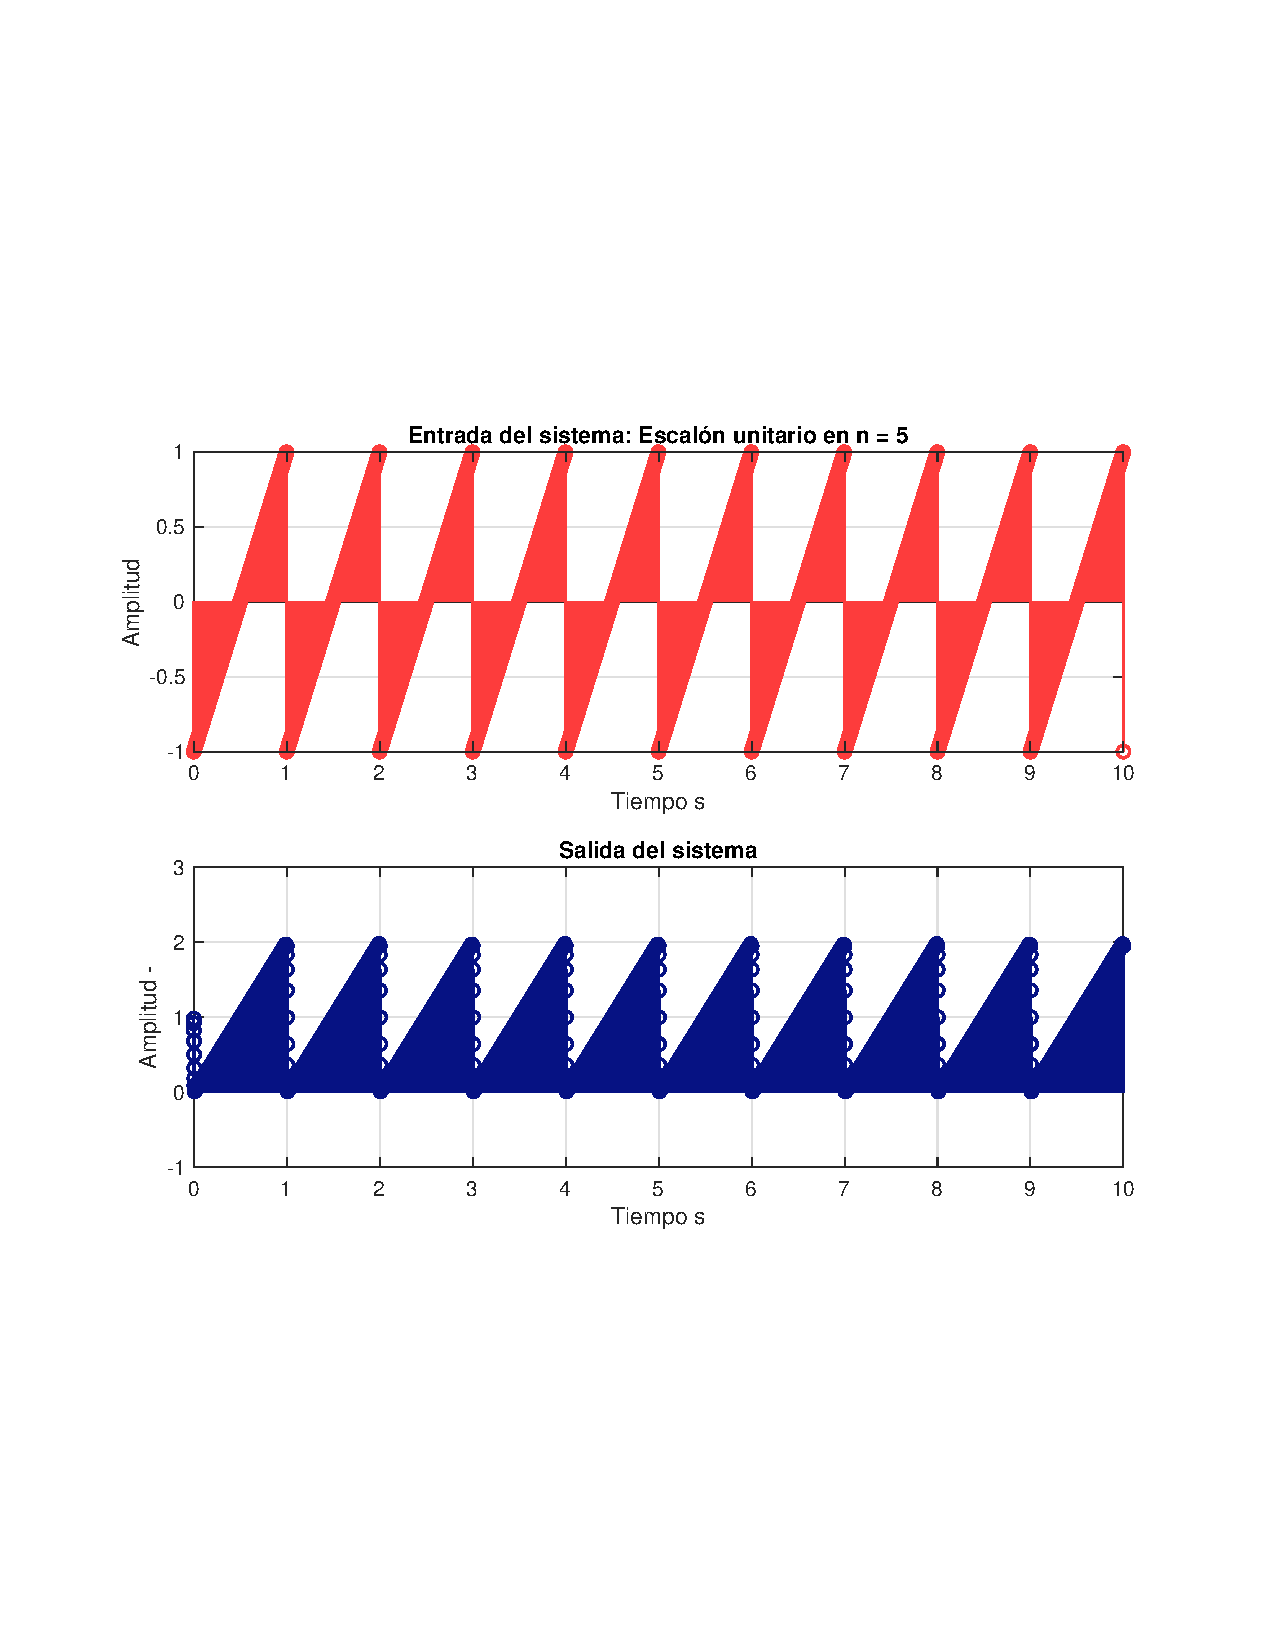
\includegraphics[width=0.6\textwidth,clip, trim = {2cm 7.0cm 2.2cm 7.0cm}]{../imgs/sistema_2_bibo_sawtooth.pdf}
				\caption{Sistema \#2, para una entrada de señal triangular \textbf{(Arriba)}, se tiene la siguiente salida \textbf{(Abajo)}.}
				\label{fig:s_2_bibo_sawtooth}
			\end{figure}
		
			Nuevamente, el resultado obtenido es idéntico, a la señal de entrada se le suma una constante, por lo que nuevamente es acotada. Tomando en consideración estos resultados, \textbf{se puede especular que el sistema es BIBO estable}.

\newpage

	\subsection{Sistema \#3}
		\subsubsection{Invariancia temporal}
			Aplicando la señal de prueba en el sistema, con retardo igual a cero: 
			\begin{figure}[H]
				\center
				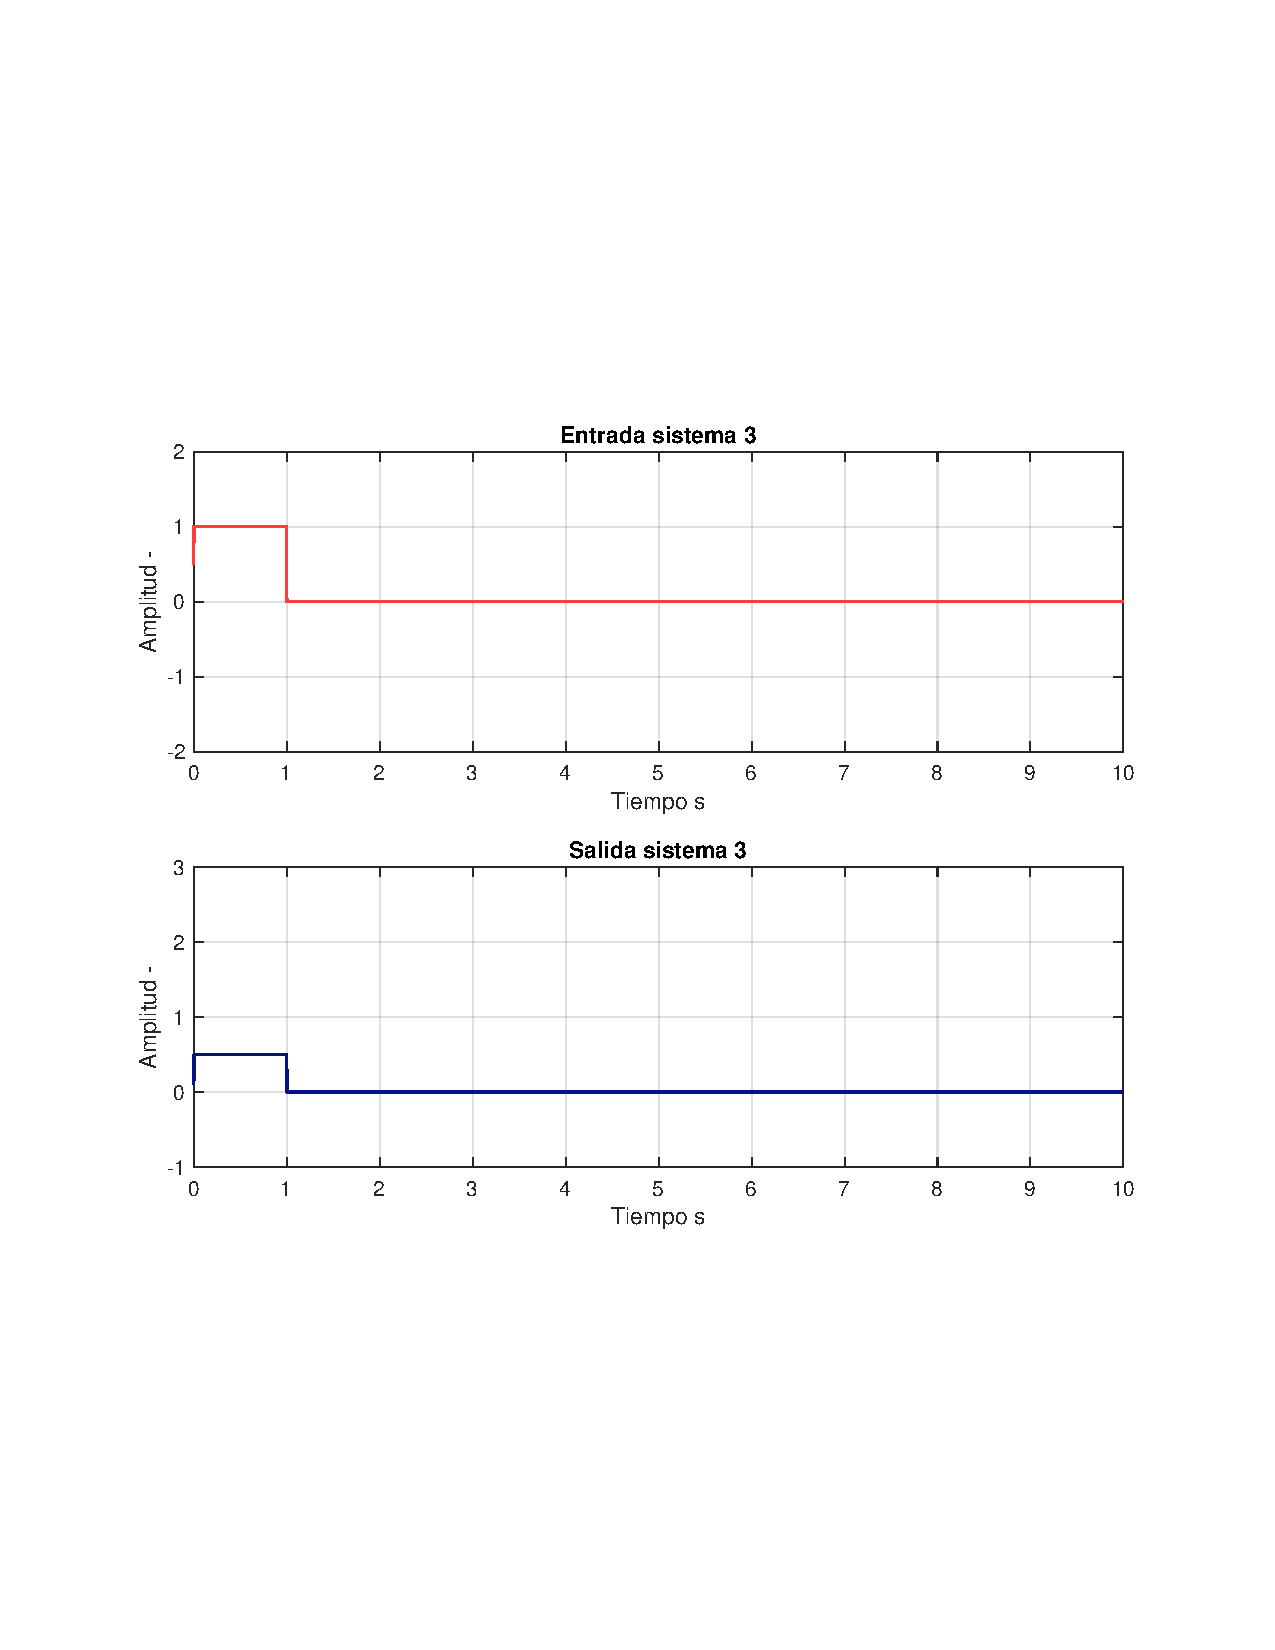
\includegraphics[width=0.6\textwidth,clip, trim = {2cm 7.0cm 2.2cm 7.0cm}]{../imgs/sistema_3_invarianza_temporal_noretardo.pdf}
				\caption{Sistema \#3 Entrada: Pulso cuadrado de duracion 1 \textit{s} \textbf{(Arriba)}. Salida del sistema \textbf{(Abajo)}.}
				\label{fig:s_3_time_invariant_test_1}
			\end{figure}
			Para un retardo de 5 s:
			\begin{figure}[H]
				\center
				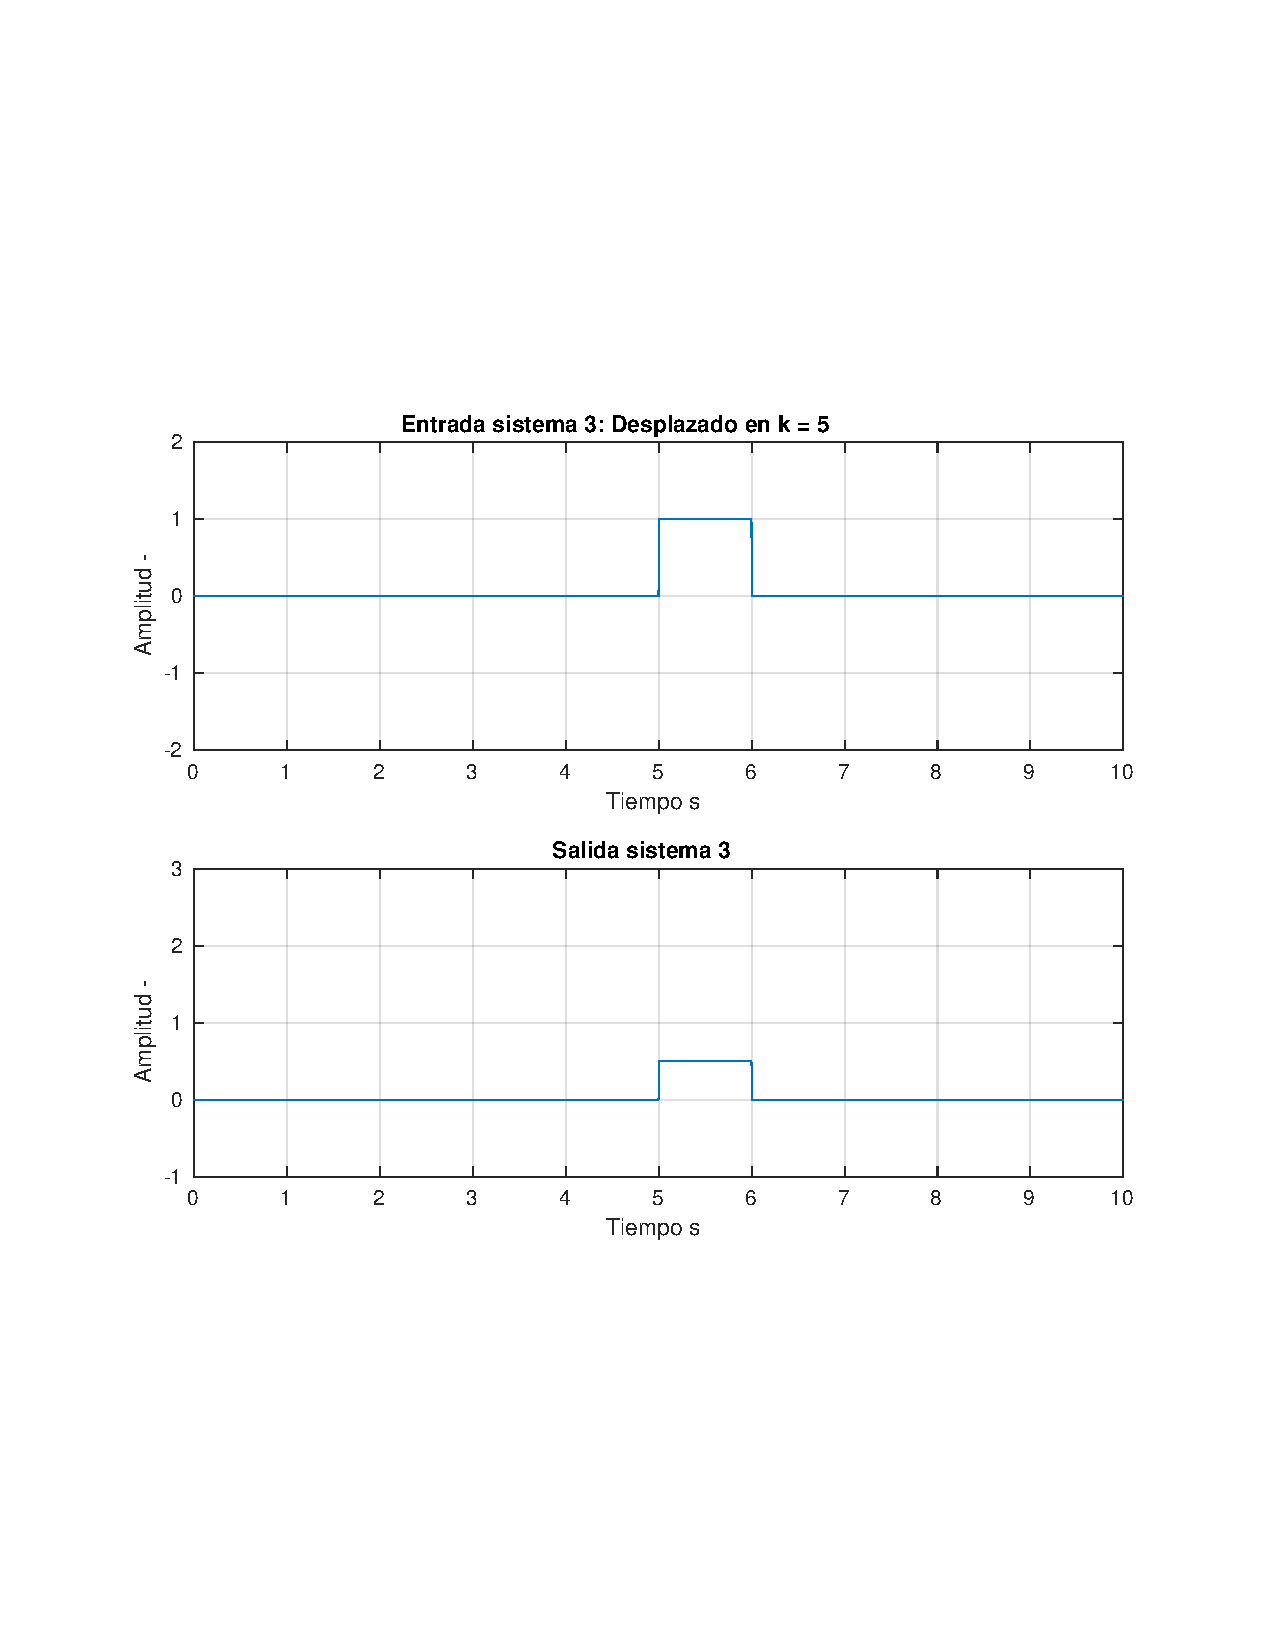
\includegraphics[width=0.6\textwidth,clip, trim = {2cm 7.0cm 2.2cm 7.0cm}]{../imgs/sistema_3_invarianza_temporal_retardo.pdf}
				\caption{Sistema \#3 Entrada: Pulso cuadrado de duracion 1 \textit{s}, desplazado en 5 \textit{s} \textbf{(Arriba)}. Salida del sistema \textbf{(Abajo)}.}
				\label{fig:s_3_time_invariant_test_2}
			\end{figure}
			
			Se obtiene la misma salida, simplemente desplazada, cumpliendo la condición de la ecuación \ref{eq:cond_invarianza_temporal}. Se puede decir que el sistema es \textbf{invariante en el tiempo}.

\newpage

		\subsubsection{Linealidad}
			Generando las entradas del sistema $u_{1}[n]$ y $u_{2}[n]$:
			\begin{figure}[H]
				\center
				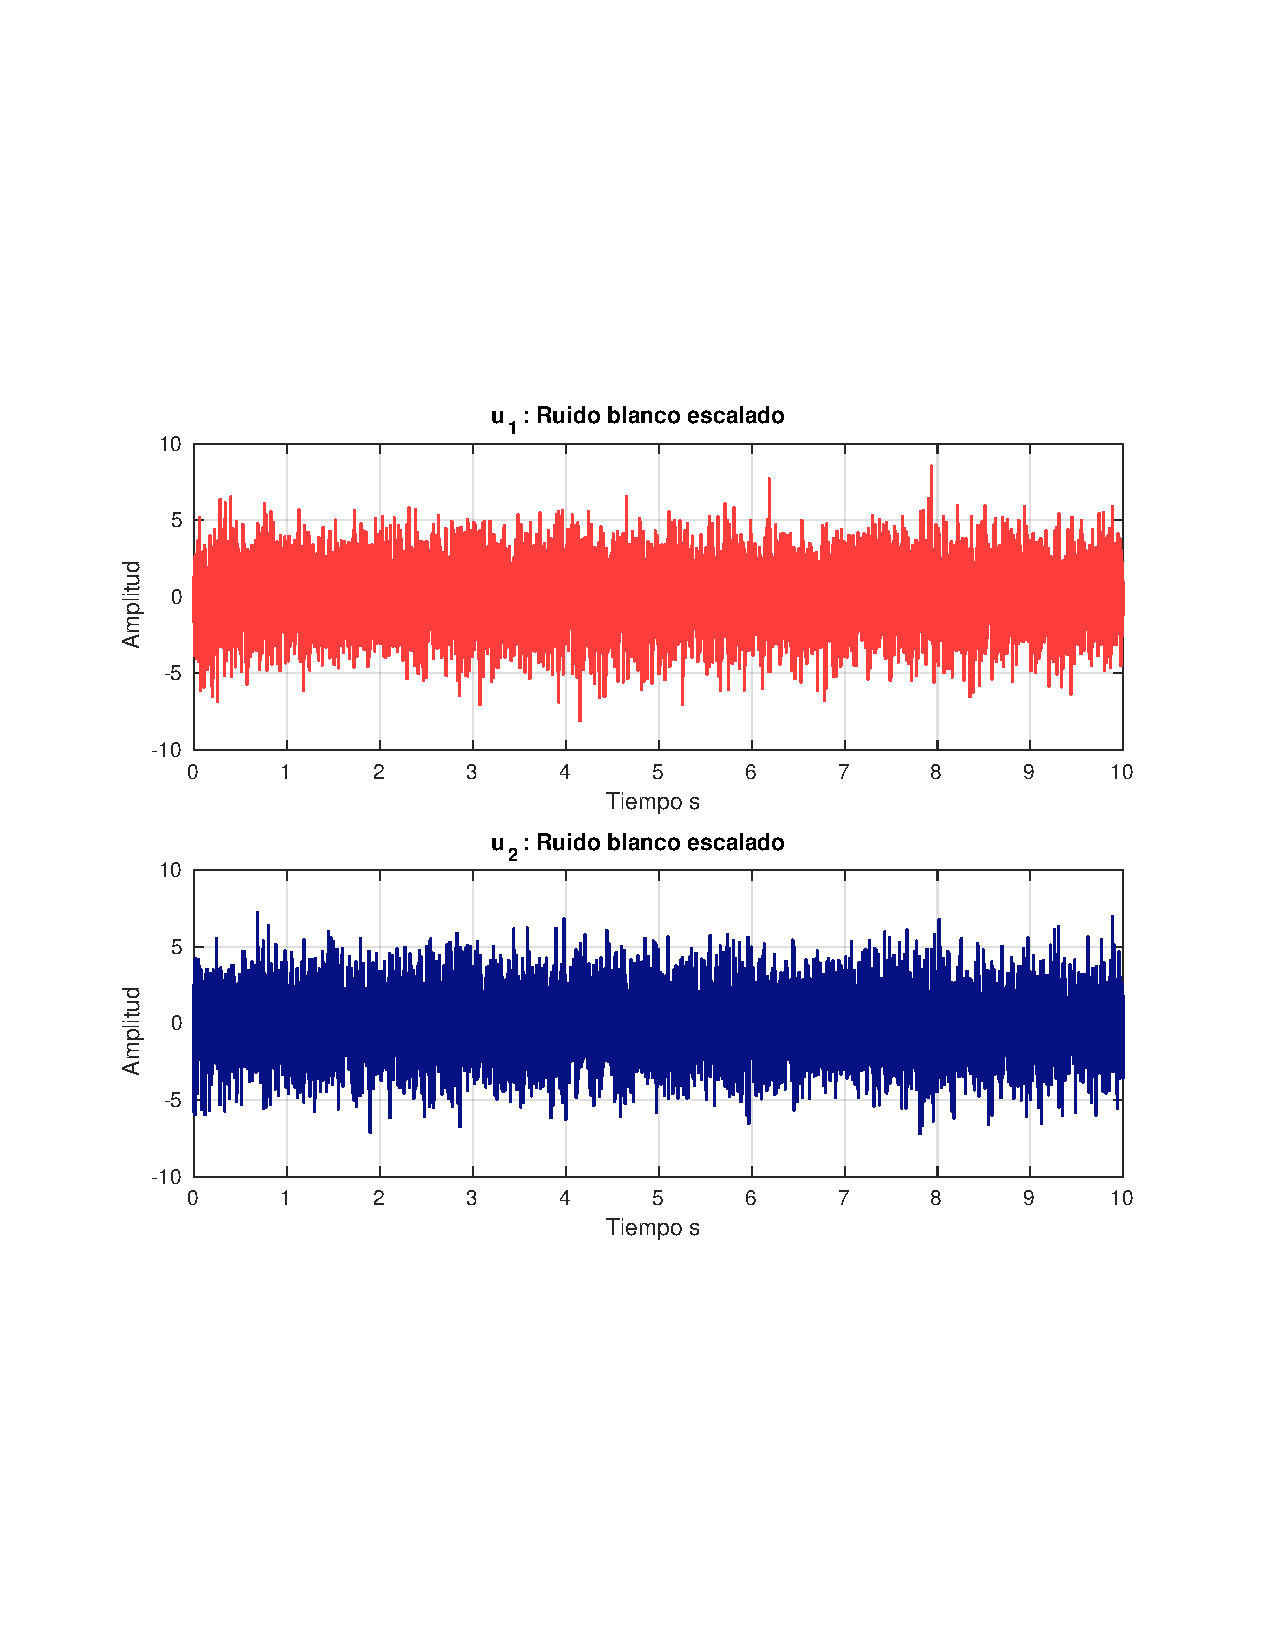
\includegraphics[width=0.6\textwidth,clip, trim = {2cm 7.0cm 2.2cm 7.0cm}]{../imgs/sistema_3_linealidad_entradas.pdf}
				\caption{Entradas del sistema}
				\label{fig:s_3_lineality_inputs}
			\end{figure}
			Comprobando las salidas del sistema:
			\begin{figure}[H]
				\center
				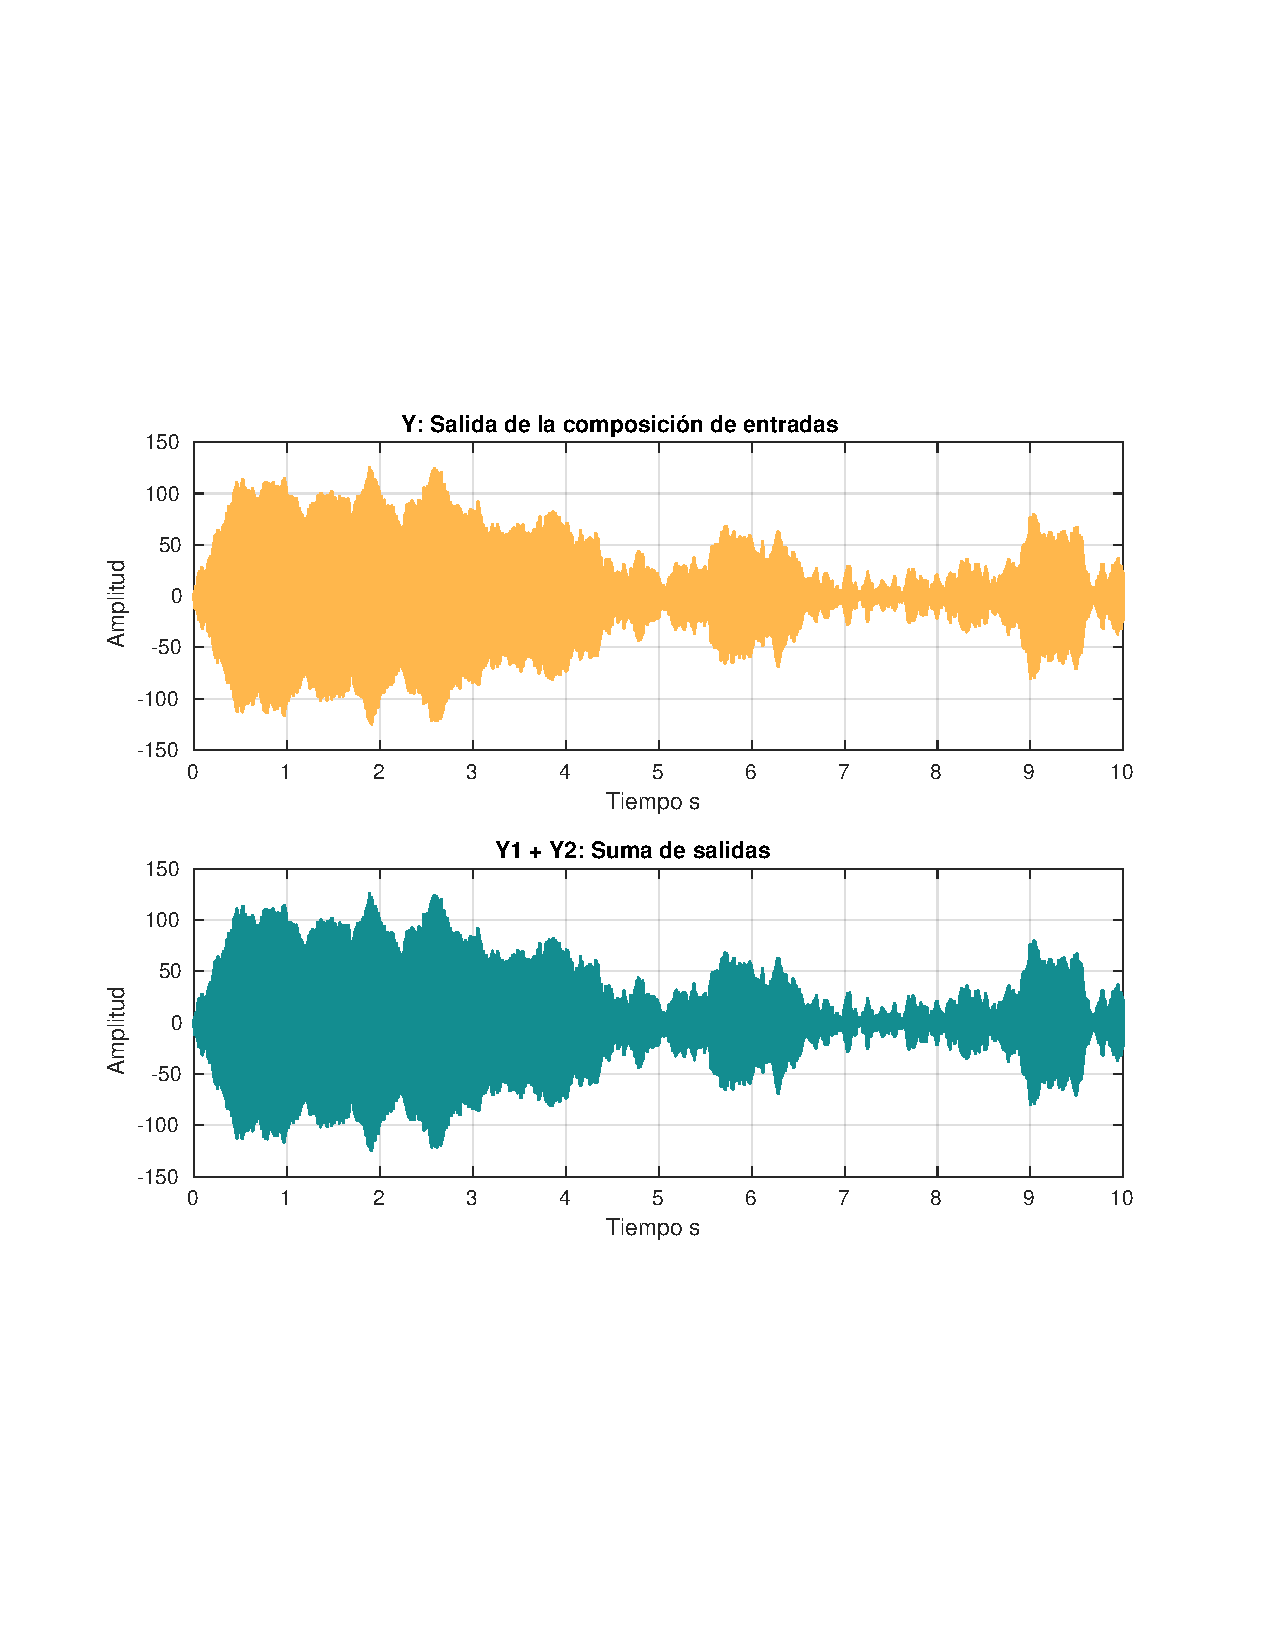
\includegraphics[width=0.6\textwidth,clip, trim = {2cm 7.0cm 2.2cm 7.0cm}]{../imgs/sistema_3_linealidad_salidas.pdf}
				\caption{Salidas del sistema: $Y[n]$ \textbf{(Arriba)}. $Y_{1}[n] + Y_{2}[n]$ \textbf{(Abajo)}.}
				\label{fig:s_3_lineality_outputs}	
			\end{figure}

\newpage			

			Realizando la comparación de salidas:
			\begin{figure}[H]
				\center
				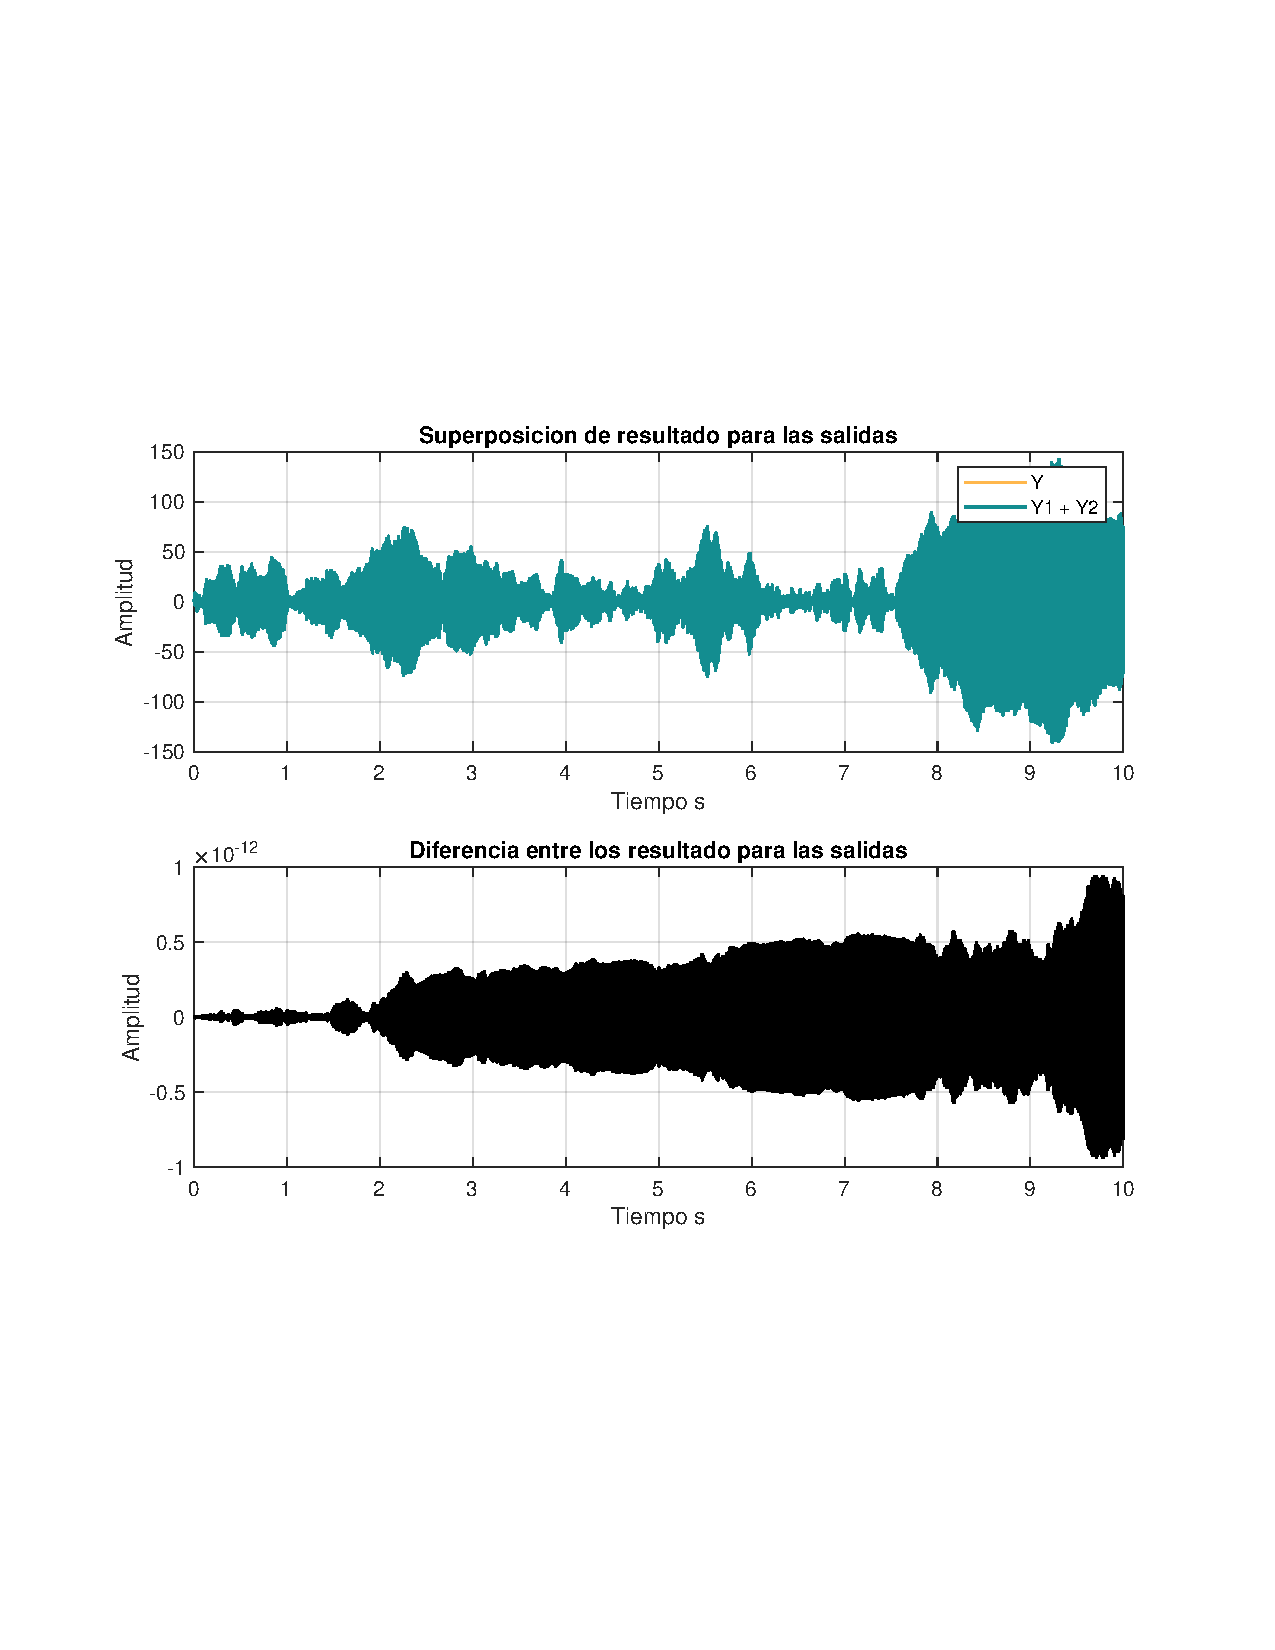
\includegraphics[width=0.6\textwidth,clip, trim = {2cm 7.0cm 2.2cm 7.0cm}]{../imgs/sistema_3_linealidad_superpuestas.pdf}
				\caption{Superposición de las señales de salida \textbf{(Arriba)}. Representación de la resta punto a punto de las señales. \textbf{(Abajo)}.}
				\label{fig:s_3_lineality_superposition}
			\end{figure}
			
			Dado el resultado obtenido en la figura \ref{fig:s_3_lineality_outputs}, ambas señales son identicas, hecho que es comprobado en la figura \ref{fig:s_3_lineality_superposition}, donde se puede comprobar que la diferencia de ambas señales es del orden de $10^{-12}$. Por lo que se puede decir que el sistema cumple \textbf{linealidad}.
			
		\subsubsection{Estabilidad BIBO}
			Aplicandole al sistema un delta de Kronecker:
		
			\begin{figure}[H]
				\center
				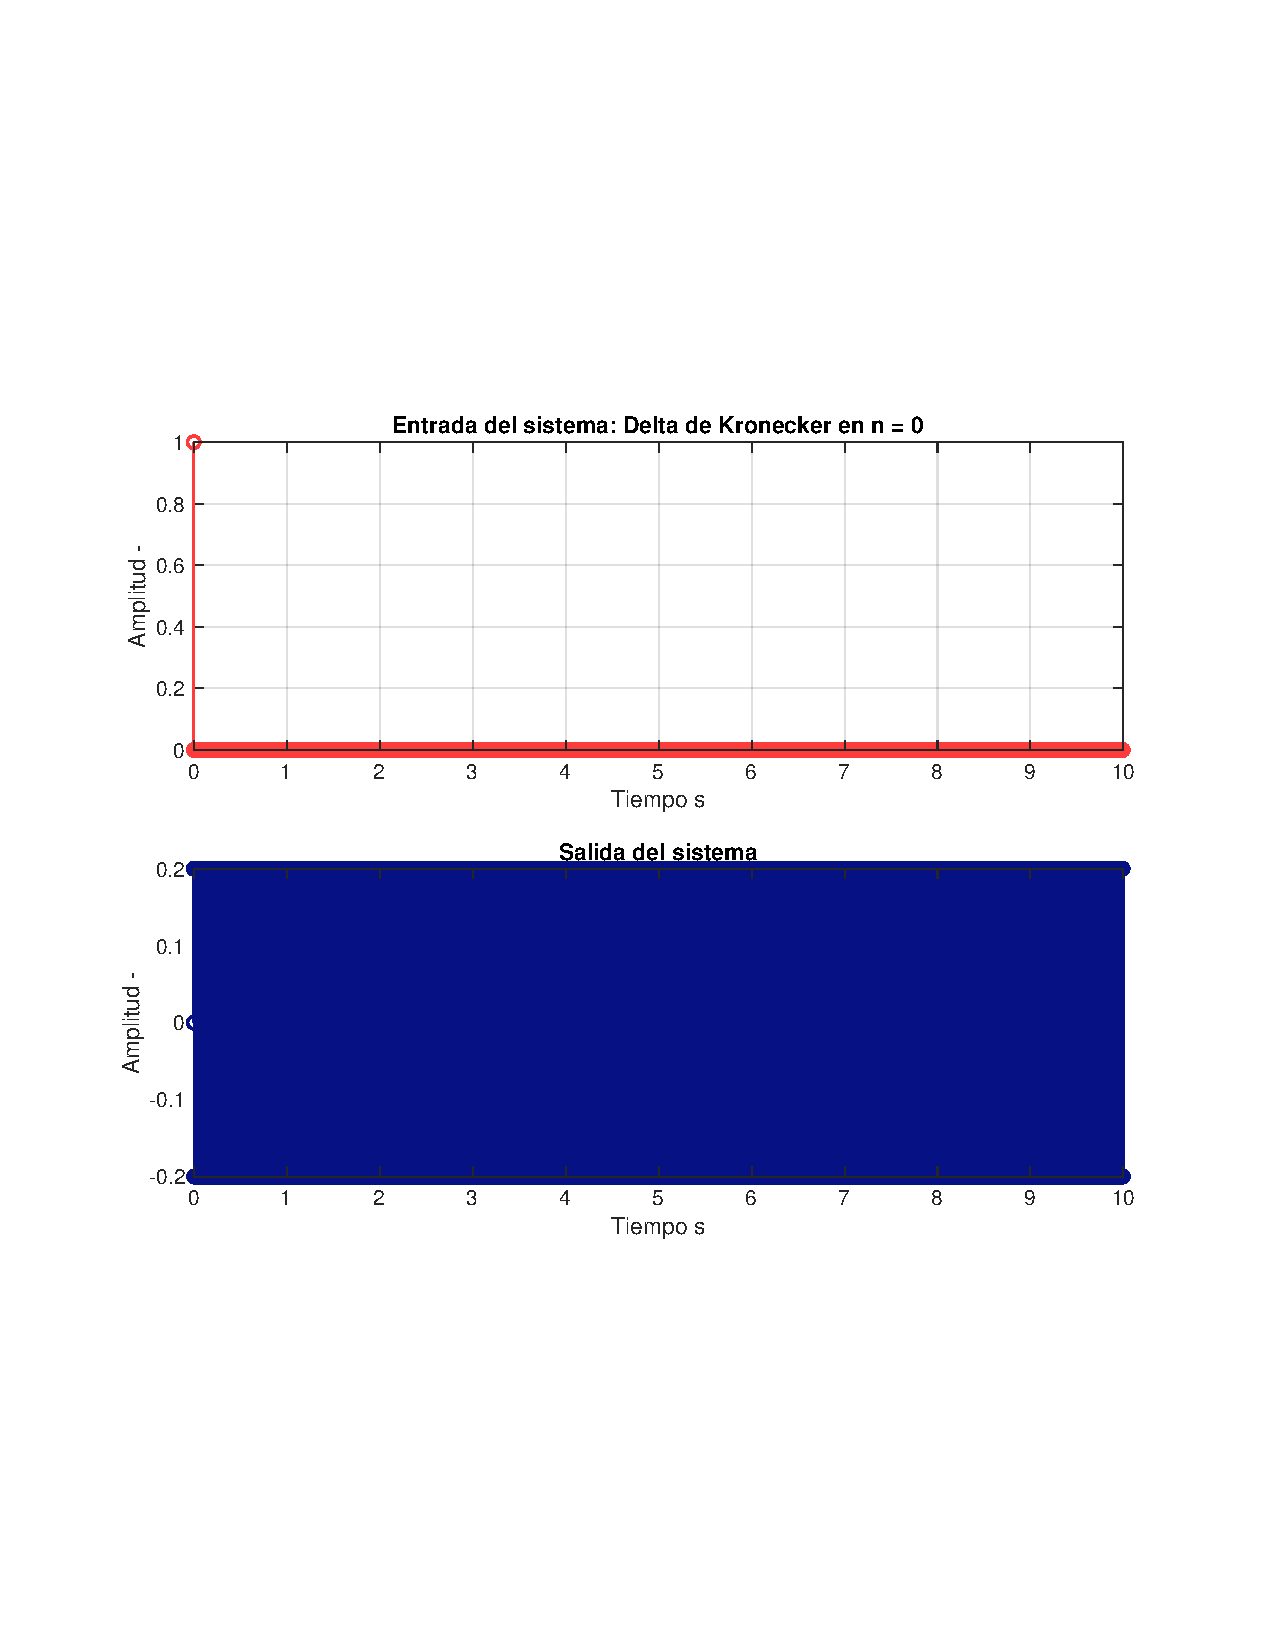
\includegraphics[width=0.6\textwidth,clip, trim = {2cm 7.0cm 2.2cm 7.0cm}]{../imgs/sistema_3_bibo_n_0.pdf}
				\caption{Sistema \#3, para una entrada de un delta de Kronecker \textbf{(Arriba)}, para la cual se tiene la siguiente respuesta \textbf{(Abajo)}.}
				\label{fig:s_3_bibo_n_0}
			\end{figure}
		
			A la salida del sistema, se obtiene una señal que se asemeja a un escalón unitario, el cual es acotado. A partir del resultado, para esta señal, podemos decir que para un delta, el sistema es estable. Procediendo a probar con un escalón unitario:
		
			\begin{figure}[H]
				\center
				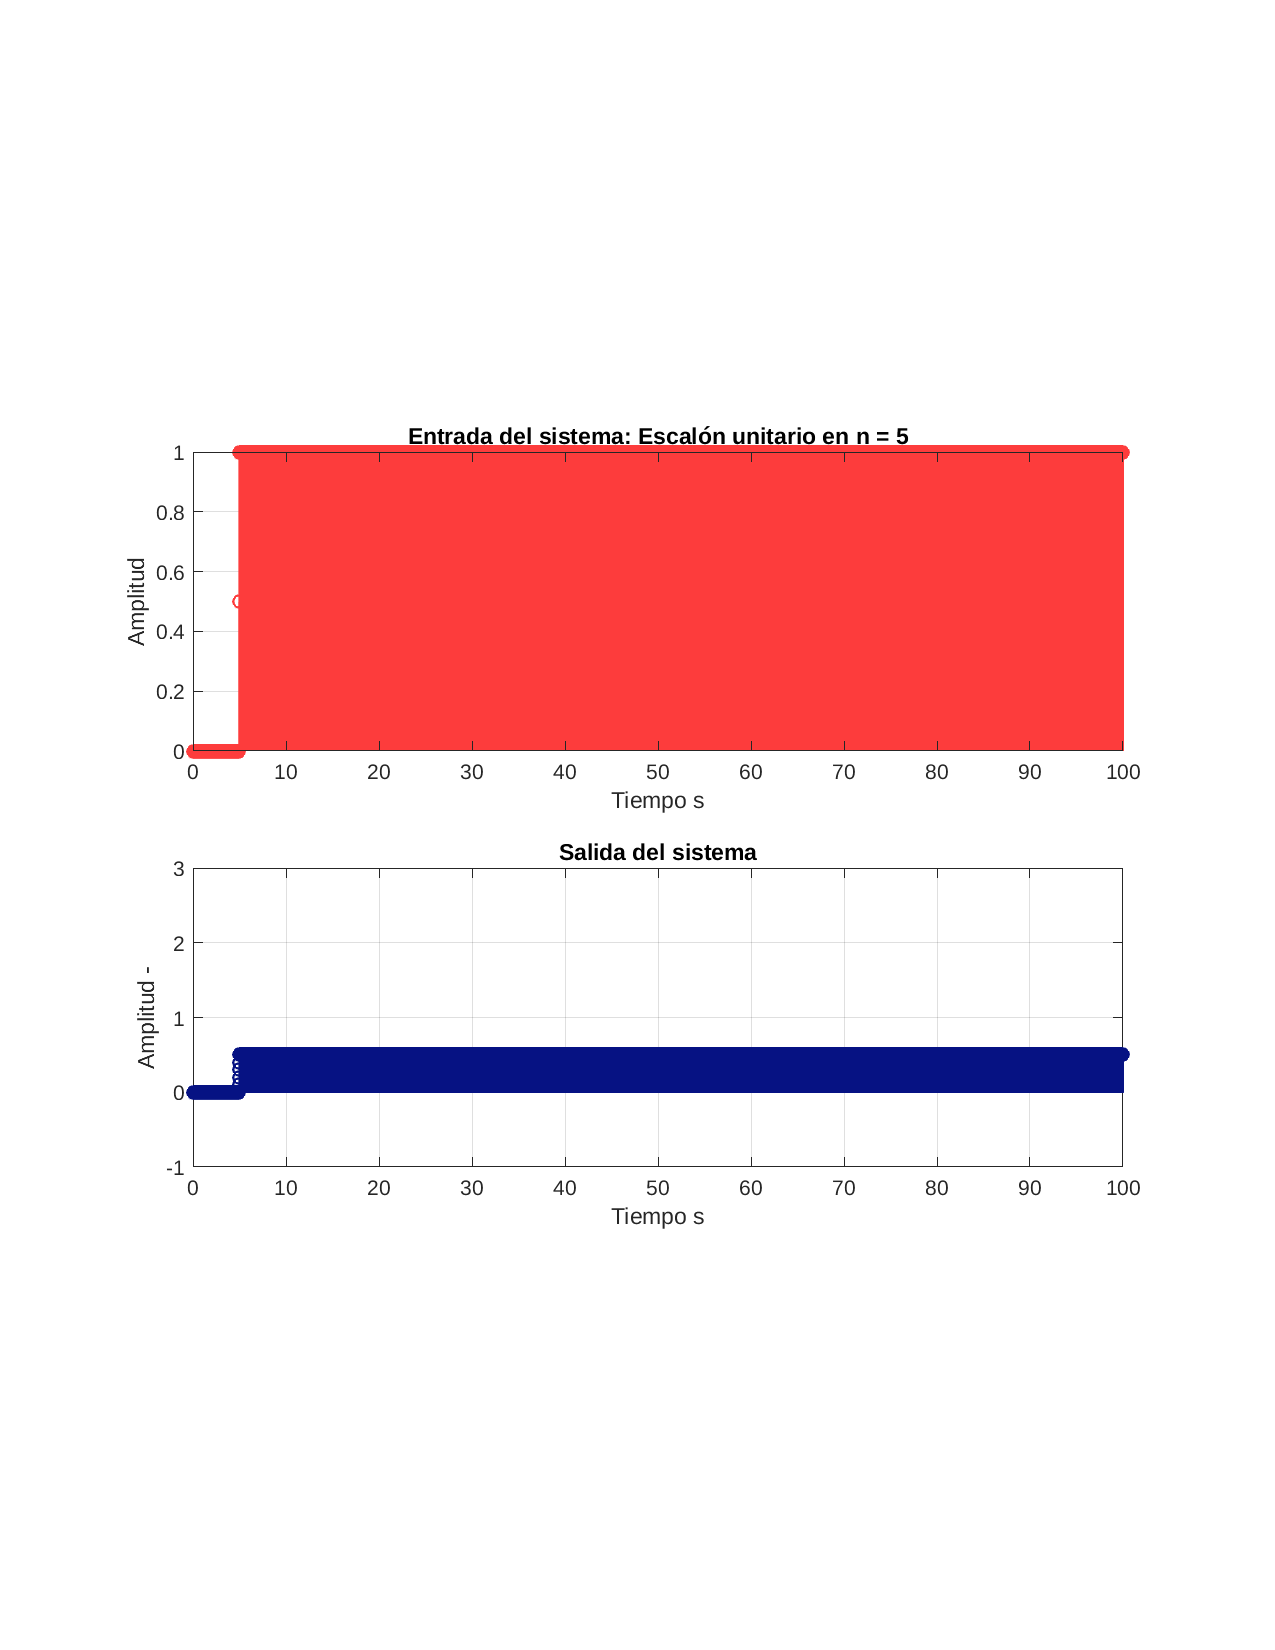
\includegraphics[width=0.6\textwidth,clip, trim = {2cm 7.0cm 2.2cm 7.0cm}]{../imgs/sistema_3_bibo_heaviside_n_5.pdf}
				\caption{Sistema \#3, para una entrada de escalón unitario, activado en n = 5 \textbf{(Arriba}}, para el cual se tiene la siguiente respuesta \textbf{(Abajo)}. 
				\label{fig:s_3_bibo_heaviside_n_5}
			\end{figure}
		
			Para esta salida,la respuesta del sistema es similar a la anterior, lo que da para especular, que el sistema mantiene la entrada que recibe, para este entrada el sistema nuevamente es estable. Siguiendo con la última señal de prueba, una señal triangular de amplitud 1 y frecuencia 1 \textit{Hz}: 
			\begin{figure}[H]
				\center
				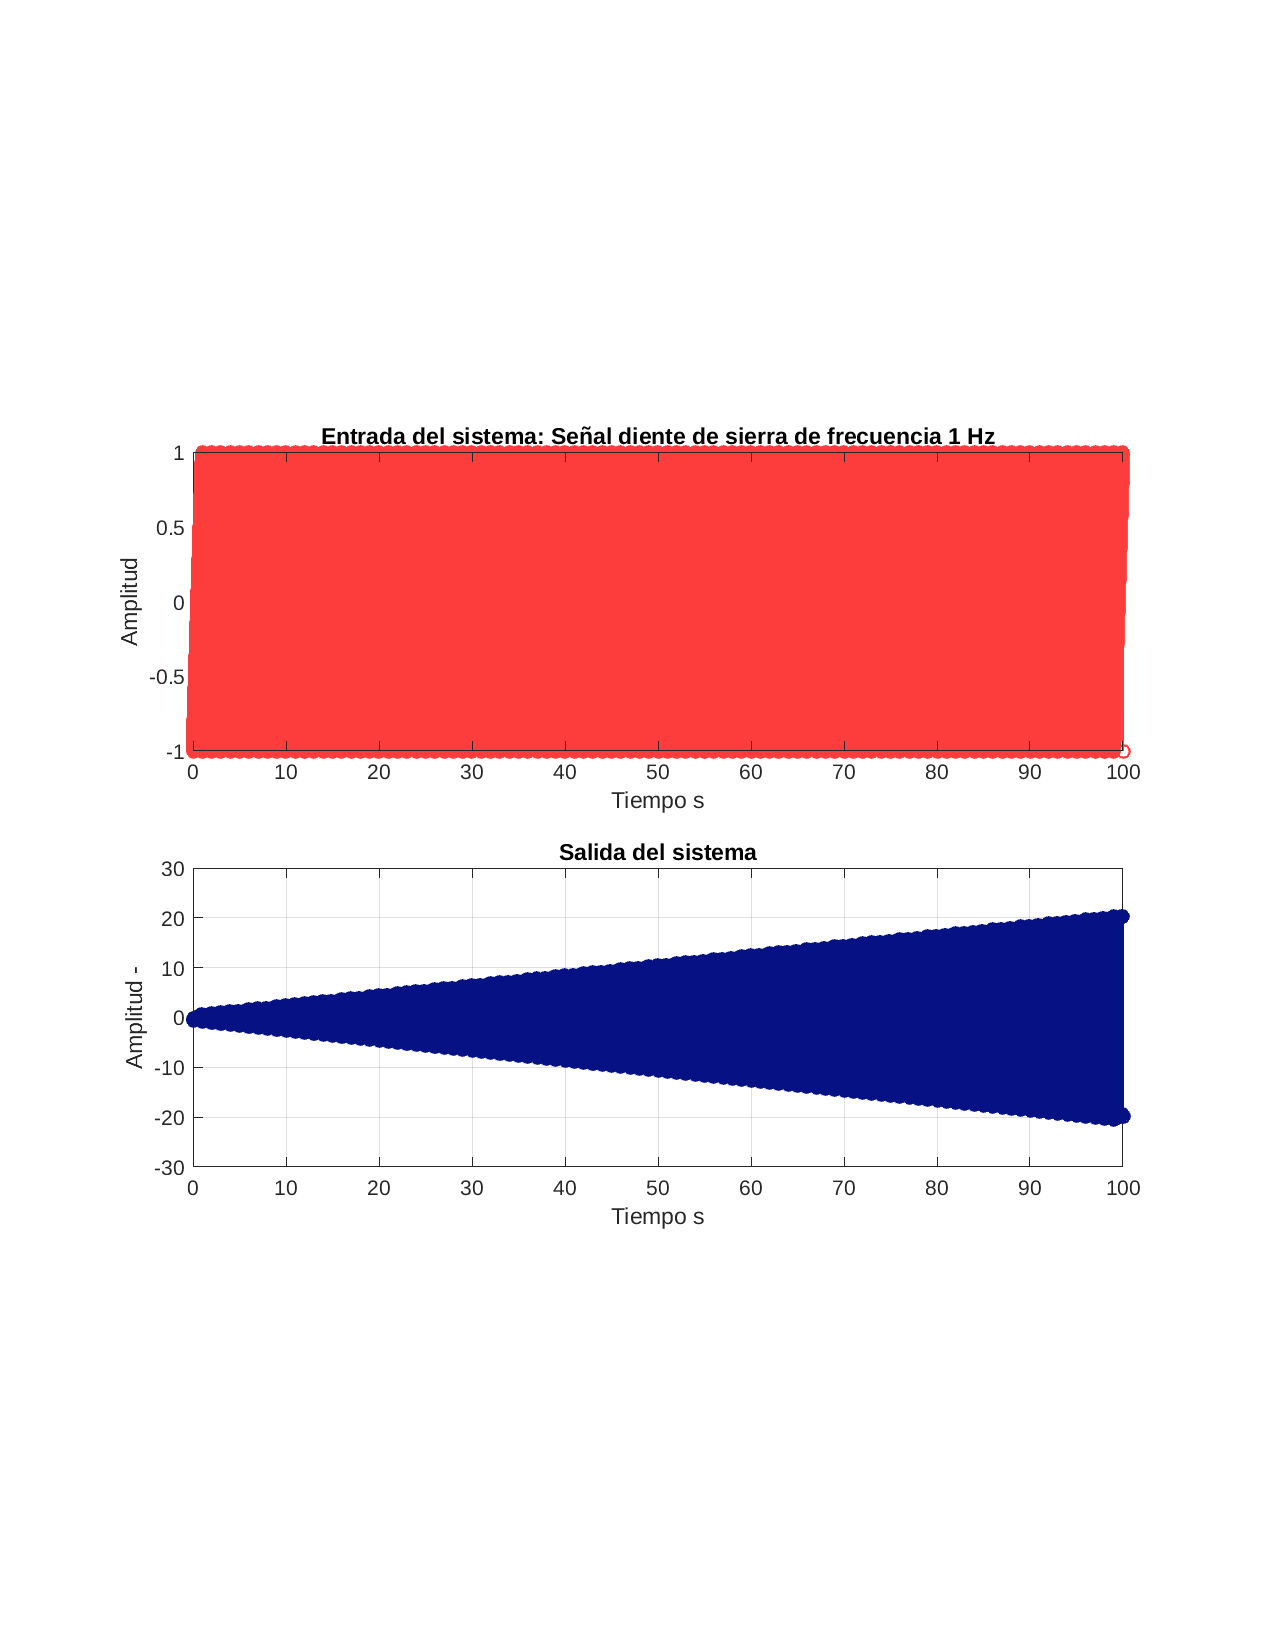
\includegraphics[width=0.6\textwidth,clip, trim = {2cm 7.0cm 2.2cm 7.0cm}]{../imgs/sistema_3_bibo_sawtooth.pdf}
				\caption{Sistema \#3, para una entrada de señal triangular \textbf{(Arriba)}, se tiene la siguiente salida \textbf{(Abajo)}.}
				\label{fig:s_3_bibo_sawtooth}
			\end{figure}
		
			Para esta entrada, el sistema tiende a amplificarse, lo que da pie a asumir, que la salida no será acotada. Por lo que se puede decir que el sistema \textbf{no es estable}.
			
	\subsection{Resumen}
		Resumiendo los resultados hallados en una tabla:
		\begin{table}[H]
			\center
			\begin{tabular}{|c|c|c|c|}
				\hline
				\textbf{Criterio} & \textbf{S1} & \textbf{S2} & \textbf{S3} \\
				\hline
				\textbf{Invariancia temporal} & No & Si & Si \\
				\hline
				\textbf{Linealidad} & Si & No & Si \\
				\hline
				\textbf{Estabilidad BIBO} & No & Si & No \\
				\hline			
			\end{tabular}
			\caption{Resumen de las características de los sistemas}
			\label{tab:summary_systems}
		\end{table}
